%-------------------------------------------------------------------------------
% This file provides a skeleton ATLAS note.
% \pdfinclusioncopyfonts=1
% This command may be needed in order to get \ell in PDF plots to appear. Found in
% https://tex.stackexchange.com/questions/322010/pdflatex-glyph-undefined-symbols-disappear-from-included-pdf
%-------------------------------------------------------------------------------
% Specify where ATLAS LaTeX style files can be found.
\newcommand*{\ATLASLATEXPATH}{latex/}
% Use this variant if the files are in a central location, e.g. $HOME/texmf.
% \newcommand*{\ATLASLATEXPATH}{}
%-------------------------------------------------------------------------------
\documentclass[NOTE, atlasdraft=true, texlive=2016, UKenglish]{\ATLASLATEXPATH atlasdoc}
\usepackage{float}
\usepackage{euler}\usepackage{pgf}
%\usepackage{subcaption}
%\usepackage{subfig}
%\usepackage{natbib}
\usepackage{geometry}
\usepackage{pdflscape}
\DeclareOldFontCommand{\bf}{\normalfont\bfseries}{\mathbf}
% The language of the document must be set: usually UKenglish or USenglish.
% british and american also work!
% Commonly used options:
%  atlasdraft=true|false This document is an ATLAS draft.
%  texlive=YYYY          Specify TeX Live version (2016 is default).
%  coverpage             Create ATLAS draft cover page for collaboration circulation.
%                        See atlas-draft-cover.tex for a list of variables that should be defined.
%  cernpreprint          Create front page for a CERN preprint.
%                        See atlas-preprint-cover.tex for a list of variables that should be defined.
%  NOTE                  The document is an ATLAS note (draft).
%  PAPER                 The document is an ATLAS paper (draft).
%  CONF                  The document is a CONF note (draft).
%  PUB                   The document is a PUB note (draft).
%  BOOK                  The document is of book form, like an LOI or TDR (draft)
%  txfonts=true|false    Use txfonts rather than the default newtx
%  paper=a4|letter       Set paper size to A4 (default) or letter.

%-------------------------------------------------------------------------------
% Extra packages:
%\usepackage{\ATLASLATEXPATH atlaspackage}
\usepackage[subfigure]{\ATLASLATEXPATH atlaspackage}
%\usepackage{\ATLASLATEXPATH atlassubfigure}
% Commonly used options:
%  biblatex=true|false   Use biblatex (default) or bibtex for the bibliography.
%  backend=bibtex        Use the bibtex backend rather than biber.
%  subfigure|subfig|subcaption  to use one of these packages for figures in figures.
%  minimal               Minimal set of packages.
%  default               Standard set of packages.
%  full                  Full set of packages.
%-------------------------------------------------------------------------------
% Style file with biblatex options for ATLAS documents.
\usepackage{\ATLASLATEXPATH atlasbiblatex}

% Package for creating list of authors and contributors to the analysis.
\usepackage{\ATLASLATEXPATH atlascontribute}

% Useful macros
\usepackage{\ATLASLATEXPATH atlasphysics}
% See doc/atlas_physics.pdf for a list of the defined symbols.
% Default options are:
%   true:  journal, misc, particle, unit, xref
%   false: BSM, heppparticle, hepprocess, hion, jetetmiss, math, process, other, texmf
% See the package for details on the options.

% Files with references for use with biblatex.
% Note that biber gives an error if it finds empty bib files.
\addbibresource{wz_heavy_flavor.bib}
\addbibresource{bib/ATLAS.bib}
\addbibresource{bib/CMS.bib}
\addbibresource{bib/ConfNotes.bib}
\addbibresource{bib/PubNotes.bib}

% Paths for figures - do not forget the / at the end of the directory name.
\graphicspath{{logos/}{figures/}}

% Add you own definitions here (file wz_heavy_flavor-defs.sty).
\usepackage{wz_heavy_flavor-defs}

%-------------------------------------------------------------------------------
% Generic document information
%-------------------------------------------------------------------------------

% Title, abstract and document 
%-------------------------------------------------------------------------------
% This file contains the title, author and abstract.
% It also contains all relevant document numbers used for an ATLAS note.
%-------------------------------------------------------------------------------

% Title
\AtlasTitle{WZ + Heavy Flavor Production in pp collisions at $\sqrt{s}$ = 13 TeV}

% Draft version:
% Should be 1.0 for the first circulation, and 2.0 for the second circulation.
% If given, adds draft version on front page, a 'DRAFT' box on top of each other page, 
% and line numbers.
% Comment or remove in final version.
\AtlasVersion{0.1}

% Abstract - % directly after { is important for correct indentation
\AtlasAbstract{%
        A measurement of WZ produced with an associated heavy flavor jet is performed using 140 $fb^{-1}$ of proton-proton collision data at $\sqrt{s} =$ 13 TeV from the ATLAS experiment at the LHC. The measurement is performed in the fully leptonic decay mode, $WZ\rightarrow l\nu ll$. The cross-section of WZ + b-jets is measured to be $X\pm X\pm X$, while the cross-section of WZ + charm is measured as X, with a correlation of X between the two processes. 
}

% Author - this does not work with revtex (add it after \begin{document})
\author{The ATLAS Collaboration}

% Authors and list of contributors to the analysis
% \AtlasAuthorContributor also adds the name to the author list
% Include package latex/atlascontribute to use this
% Use authblk package if there are multiple authors, which is included by latex/atlascontribute
% \usepackage{authblk}
% Use the following 3 lines to have all institutes on one line
% \makeatletter
% \renewcommand\AB@affilsepx{, \protect\Affilfont}
% \makeatother
% \renewcommand\Authands{, } % avoid ``. and'' for last author
% \renewcommand\Affilfont{\itshape\small} % affiliation formatting
% \AtlasAuthorContributor{First AtlasAuthorContributor}{a}{Author's contribution.}
% \AtlasAuthorContributor{Second AtlasAuthorContributor}{b}{Author's contribution.}
% \AtlasAuthorContributor{Third AtlasAuthorContributor}{a}{Author's contribution.}
% \AtlasContributor{Fourth AtlasContributor}{Contribution to the analysis.}
% \author[a]{First Author}
% \author[a]{Second Author}
% \author[b]{Third Author}
% \affil[a]{One Institution}
% \affil[b]{Another Institution}

% If a special author list should be indicated via a link use the following code:
% Include the two lines below if you do not use atlasstyle:
% \usepackage[marginal,hang]{footmisc}
% \setlength{\footnotemargin}{0.5em}
% Use the following lines in all cases:
% \usepackage{authblk}
% \author{The ATLAS Collaboration%
% \thanks{The full author list can be found at:\newline
%   \url{https://atlas.web.cern.ch/Atlas/PUBNOTES/ATL-PHYS-PUB-2017-007/authorlist.pdf}}
% }

% ATLAS reference code, to help ATLAS members to locate the paper
\AtlasRefCode{GROUP-2017-XX}

% ATLAS note number. Can be an COM, INT, PUB or CONF note
% \AtlasNote{ATLAS-CONF-2017-XXX}
% \AtlasNote{ATL-PHYS-PUB-2017-XXX}
% \AtlasNote{ATL-COM-PHYS-2017-XXX}

% Author and title for the PDF file
\hypersetup{pdftitle={ATLAS document},pdfauthor={The ATLAS Collaboration}}

%-------------------------------------------------------------------------------
% Content
%-------------------------------------------------------------------------------
\begin{document}

\maketitle

\tableofcontents

% List of contributors - print here or after the Bibliography.
%\PrintAtlasContribute{0.30}
\clearpage

%------------------------------------------------------------------------------
\section{Changes and outstanding items}
\label{sec:changes}
%------------------------------------------------------------------------------

\subsection{Changelog}

This is version 3

\subsubsection{Changes relative to v2}

\begin{itemize}
    \item Included a section on tZ interference effects, \ref{subsec:interference}. 
    \item 
\end{itemize}

\subsubsection{Changes relative to v1}

\begin{itemize}
    \item Added GRL list
    \item Fixed latex issue in line 92, typo in line 172
    \item Added tables \ref{tbl:selection} and \ref{tbl:tightleps}, summarizing the event and object selection
    \item Added table \ref{tab:dsids}, which includes the DSID of samples used
    \item Included reference to WZ inclusive paper in introduction
\end{itemize}

\subsection{Outstanding Items}

\begin{itemize}
    \item Include new Madgraph WZjj VBS samples - currently using Sherpa, which is missing b-jet diagrams
    \item Move to updated 2018 data and MC recommendations
    \item Understand data/MC discrepancies, likely from fake contribution. Possibly move to data driven fakes
    \item Investigate VVV samples, ensure no overlap with WZjj samples
    \item Include selection to reject events with a fourth soft lepton to reduce ZZ->llll contribution
    \item Add details on top mass reconstruction, specifically to justify choices made
\end{itemize}



\clearpage

%-------------------------------------------------------------------------------
\section{Introduction}
\label{sec:intro}
%-------------------------------------------------------------------------------

The production of $WZ$ in association with a heavy flavor jet represents an important background for many major analyses. This includes any process with leptons and b-jets in the final state, such as $t\bar{t}H$, $t\bar{t}W$, and $t\bar{t}Z$. While precise measurements have been made of $WZ$ production \cite{WZ_36}, $WZ$ + heavy flavor remains poorly understood. This is largely because the QCD processes involved in the production of the b-jet make it difficult to simulate accurately. This introduces a large uncertainty for analyses that include this process as a background.  

Motivated by its relevance to the $t\bar{t}H$ multilepton analysis, we perform a study of the fully leptonic decay mode of this channel, that is, events where both the W and Z decay leptonically. This gives a final state signature of three leptons and at least one jet.

Events with three leptons and one or two jets are sorted into pseudo-continuous b-tagging regions based on the MV2c10 b-tag score of their associated jets. This is done to separate $WZ$ + b-jet events from $WZ$ + charm and $WZ$ + light jets. These regions are fit to data in order make a more accurate estimate of the contribution of $WZ$ + heavy-flavor, where heavy-flavor jets include b-jets and charm jets. The full Run-2 dataset collected by the ATLAS detector, representing 139 $fb^{-1}$ of data from pp collisions at $\sqrt{s} = 13$ TeV, is used for this study.

Section \ref{sec:data} details the data and Monte Carlo (MC) samples used in the analysis, and the reconstruction of various physics objects is described in section \ref{sec:obj}. Section \ref{sec:evt_selection} describes the event selection applied to these samples. The multivariate analysis techniques used to separate the tZ background from WZ + heavy flavor are described in section \ref{sec:tZ_bdt}. The regions defined for the fit are then described in section \ref{sec:signal_region}. Section \ref{sec:sys} describes the various sources of systematic uncertainties considered in the fit. Finally, the results of the analysis are summarized in section \ref{sec:results}, followed by a brief conclusion in section \ref{sec:conclusion}.

\textbf{The current state of the analysis shows blinded results for the full 2018 dataset, awaiting unblinding approval. 2018 recommendations and working points have not yet been fully implemented, and the 2018 dataset contributions currently use 2017 recommendations.}

%-------------------------------------------------------------------------------
\section{Data and Monte Carlo Samples}
\label{sec:data}
%-------------------------------------------------------------------------------

Both data and Monte Carlo samples used in this analysis were prepared in the \verb|xAOD| format, which was used to produce a \verb|DxAOD| sample in the \verb|HIGG8D1| derivation framework. The \verb|HIGG8D1| framework is designed for the $t\bar{t}H$ multi-lepton| analysis, which targets events with multiple leptons as well as tau hadrons. This framework skims the dataset to remove unneeded variables as well as entire events. Events are removed from the derivations that do not meet the following selection:

\begin{itemize}
    \item at least two light leptons within a range $|\eta|$<2.6, with leading lepton $p_{T}$ > 15 GeV and subleading lepton $p_{T}$ > 5 GeV
    \item at least one light lepton with $p_{T}$ > 15 GeV within a range $|\eta|$<2.6, and at least two hadronic taus with $p_{T}$ > 15 GeV.
\end{itemize}

Samples were then generated from these \verb|HIGG8D1| derivations using a modified version of AnalysisTop version 21.2.36.

\subsection{Data Samples}

The study uses a sample of proton-proton collision data collected by the ATLAS detector from 2015 through 2018 at an energy of $\sqrt{s} = 13$ TeV, which represents an integrated luminosity of 140 $fb^{-1}$. The data set was collected with a bunch crossing rate of 25 ns. All data used in this analysis was verified by data quality checks, having been included in the following Good Run Lists: 
\begin{itemize}
    \item data15\_13TeV.periodAllYear\_DetStatus-v79-repro20-02\_DQDefects-00-02-02\\\_PHYS\_StandardGRL\_All\_Good\_25ns.xml
    \item data16\_13TeV.periodAllYear\_DetStatus-v88-pro20-21\_DQDefects-00-02-04\\\_PHYS\_StandardGRL\_All\_Good\_25ns.xml 
    \item data17\_13TeV.periodAllYear\_DetStatus-v97-pro21-13\_Unknown\_PHYS\_StandardGRL\\\_All\_Good\_25ns\_Triggerno17e33prim.xml 
    \item data18\_13TeV.periodAllYear\_DetStatus-v102-pro22-04\_Unknown\_PHYS\_StandardGRL\\\_All\_Good\_25ns\_Triggerno17e33prim.xml
\end{itemize}

\subsection{Monte Carlo Samples}

Several different generators were used to produce Monte Carlo simulations of the signal and background processes. For all samples, the response of the ATLAS detector is simulated using Geant4. The WZ signal samples are simulated using Sherpa 2.2.2 \cite{sherpa}. Specific information about the Monte Carlo samples being used can be found in table \ref{tbl:evgen}.


\begin{table}[H]
\begin{center}
\caption{\label{tbl:evgen} The configurations used for event generation of signal and background processes, including the event generator, matrix element (ME) order, parton shower algorithm, and parton distribution functin (PDF). }
 \resizebox{\textwidth}{!}{
\begin{tabular}{llllll}
\hline\hline
Process & Event generator & ME order & Parton Shower & PDF   \\
\hline
$VV$, & \textsc{Sherpa} 2.2.2
& MEPS NLO & \textsc{Sherpa} & CT10 \\
$t Z$ & \textsc{MG5\_aMC} & LO & \textsc{Pythia} 6  & CTEQ6L1  \\
$\ttbar W$ & \textsc{MG5\_aMC} & NLO & \textsc{Pythia} 8 & NNPDF 3.0 NLO \\
& (\textsc{Sherpa} 2.1.1) & (LO multileg) & (\textsc{Sherpa}) & (NNPDF 3.0 NLO)  \\
$\ttbar (Z/\gamma^* \to ll)$ & \textsc{MG5\_aMC} & NLO & \textsc{Pythia} 8 & NNPDF 3.0 NLO  \\
$t\bar{t}H$ & \textsc{MG5\_aMC} & NLO & \textsc{Pythia} 8\ & NNPDF 3.0 NLO \cite{Ball:2014uwa} \\
     & (\textsc{MG5\_aMC}) & (NLO) & (\textsc{Herwig++}) & (CT10 \cite{ct10})  \\
$tHqb$ & \textsc{MG5\_aMC} & LO & \textsc{Pythia} 8 & CT10  \\
$tHW$ & \textsc{MG5\_aMC} & NLO & \textsc{Herwig++}  & CT10  \\
& (\textsc{Sherpa} 2.1.1) & (LO multileg) & (\textsc{Sherpa}) & (NNPDF 3.0 NLO)  \\
$t W Z$ & \textsc{MG5\_aMC} & NLO & \textsc{Pythia} 8 & NNPDF 2.3 LO   \\
$t\bar t t$, $t\bar t t\bar t$ & \textsc{MG5\_aMC} & LO & \textsc{Pythia} 8 & NNPDF 2.3 LO  \\
$t\bar t W^+ W^-$ & \textsc{MG5\_aMC} & LO & \textsc{Pythia} 8 & NNPDF 2.3 LO\\
$\ttbar$ & \textsc{Powheg-BOX v2} \cite{powhegtt} & NLO & \textsc{Pythia} 8 & NNPDF 3.0 NLO  \\
$\ttbar\gamma$ & \textsc{MG5\_aMC} & LO & \textsc{Pythia} 8 & NNPDF 2.3 LO \\
$s$-, $t$-channel, & \textsc{Powheg-BOX v1} \cite{powhegstp}& NLO & \textsc{Pythia} 6 & CT10 \\
 $Wt$ single top & & & &  \\
$qqVV$, $VVV$ & &   \\
$Z \to l^+l^-$ & \textsc{Sherpa} 2.2.1 & MEPS NLO  & \textsc{Sherpa} & NNPDF 3.0 NLO \\
\hline\hline
\end{tabular}
}
\end{center}
\end{table}

\begin{table}[]
    \centering
    \begin{tabular}{l|l}
        \hline\hline
        Sample & DSID \\
        \hline\hline
        $WZ$ & 364253, 364739-42 \\
        $VV$ & 364250, 364254, 364255, 363355-60, 364890 \\
        $t\bar{t}W$ & 410155 \\
        $t\bar{t}Z$ & 410156, 410157, 410218-20 \\
        low mass $t\bar{t}Z$ & 410276-8 \\
        Rare Top & 410397, 410398, 410399 \\
        single Top & 410658-9, 410644-5 \\
        three Top & 304014 \\
        four Top & 410080 \\
        $t\bar{t}WW$ & 410081 \\
        Z + jets & 364100-41 \\
        low mass Z + jets & 364198-215 \\
        W + jets & 364156-97 \\
        $V\gamma$ & 364500-35 \\
        $tZ$  & 410560 \\
        $tW$  & 410013-4 \\
        $WtZ$ & 410408 \\
        $VVV$ & 364242-9 \\
        $VH$ & 342284-5 \\
        $WtH$ & 341998 \\
        $t\bar{t}\gamma$ & 410389 \\
        $t\bar{t}$ & 410470 \\
        $t\bar{t}H$ & 345873-5, 346343-5 \\
        \hline\hline
    \end{tabular}
    \caption{List of Monte Carlo samples by data set ID used in the analysis.}
    \label{tab:dsids}
\end{table}


%-------------------------------------------------------------------------------
\section{Object Reconstruction}
\label{sec:obj}
%-------------------------------------------------------------------------------

All regions defined in this analysis share a common lepton, jet, and overall event selection. This selection is detailed here; the selection used to define the various fit regions is described in section \ref{sec:signal_region}.

\subsection{Trigger}

Events are required to be selected by dilepton triggers, as summarized in table \ref{tbl:trigger}. \textbf{The 2018 trigger has not yet been implemented, and 2018 data currently uses 2017 triggers.}

\begin{table}[h!]
 \begin{center}
   \begin{tabular}{cc}
     \toprule
                  & Dilepton triggers (2015) \\
     \midrule
      $\mu\mu$ (asymm.)          & \verb!HLT_mu18_mu8noL1! \\
      $ee$ (symm.)               & \verb!HLT_2e12_lhloose_L12EM10VH! \\
      $e\mu,\mu e$ ($\sim$symm.) & \verb!HLT_e17_lhloose_mu14! \\
     \bottomrule
                       & Dilepton triggers (2016) \\
     \midrule
      $\mu\mu$ (asymm.)                   & \verb!HLT_mu22_mu8noL1! \\
      $ee$ (symm.)                        & \verb!HLT_2e17_lhvloose_nod0! \\
      $e\mu,\mu e$ ($\sim$symm.)          & \verb!HLT_e17_lhloose_nod0_mu14! \\
     \bottomrule

                  & Dilepton triggers (2017) \\
     \midrule
      $\mu\mu$ (asymm.)                   & \verb!HLT_mu22_mu8noL1! \\
      $ee$ (symm.)                        & \verb!HLT_2e24_lhvloose_nod0! \\
      $e\mu,\mu e$ ($\sim$symm.)          & \verb!HLT_e17_lhloose_nod0_mu14! \\
     \bottomrule
   \end{tabular}
   \caption{\label{tbl:trigger} List of lowest $p_{T}$-threshold, un-prescaled dilepton triggers used for 2015-2017 data taking.}
 \end{center}
\end{table}

\subsection{Light leptons}
\label{subsec:leps}

Electron candidates are reconstructed from energy clusters in the electromagnetic calorimeter that are associated with charged particle tracks reconstructed in the inner detector~\cite{ATLAS-CONF-2016-024}.  Electron candidates are required to have $\pt > 10$ GeV and $|\eta_\textrm{cluster}| < 2.47$. Candidates in the transition region between different electromagnetic calorimeter components, $1.37 < |\eta_\textrm{cluster}| < 1.52$, are rejected. A multivariate likelihood discriminant combining shower shape and track information is used to distinguish real electrons from hadronic showers (fake electrons). To further reduce the non-prompt electron contribution, the track is required to be consistent with originating from the primary vertex; requirements are imposed on the transverse impact parameter significance ($|d_0|/\sigma_{d_0}$) and the longitudinal impact parameter ($|\Delta z_0 \sin \theta_\ell|$), as shown in table \ref{tbl:tightleps}. 
                   
Muon candidates are reconstructed by combining inner detector tracks with track segments or full tracks in the muon spectrometer \cite{PERF-2014-05}. Muon candidates are required to have $\pt > 10$~GeV and $|\eta| < 2.5$. 

All leptons are required to be isolated, and pass a non-prompt BDT selection described in detail in \cite{ttH_paper}. 

\begin{table}
\begin{center}
 \begin{tabular}{l|cccccc}
 \hline\hline
 & \multicolumn{3}{c|}{$e$} & \multicolumn{3}{c}{$\mu$} \\
 \hline
 & L & L* & T & L & L* & T \\
  \hline
  FixedCutLoose           &  No & \multicolumn{2}{|c|}{Yes} & No & \multicolumn{2}{|c}{Yes} \\
  \hline
  Non-prompt lepton BDT   &  \multicolumn{2}{c|}{No} & \multicolumn{1}{c|}{Yes} & \multicolumn{2}{c|}{No} & \multicolumn{1}{c}{Yes} \\
  \hline
  Identification  & \multicolumn{2}{c|}{Loose} & \multicolumn{1}{c|}{Tight} & \multicolumn{2}{c}{Loose} & Medium\\
  \hline
  Charge mis-assignment veto &  \multicolumn{2}{c|}{No} & Yes & \multicolumn{3}{|c}{N/A} \\
  \hline
  ambiguity bit == 0 &  \multicolumn{2}{c|}{No} & Yes & \multicolumn{3}{|c}{N/A} \\
  \hline
  Transverse impact parameter significance  &  \multicolumn{3}{c|}{$<5$} & \multicolumn{3}{c}{$<3$ } \\
  $|d_0|/\sigma_{d_0}$ & \multicolumn{3}{c|}{} &  \multicolumn{3}{c}{}  \\
  \hline
  Longitudinal impact parameter &  \multicolumn{6}{c}{$< 0.5$ mm} \\
  $|z_0 \sin \theta|$ &  \multicolumn{6}{c}{} \\
  \hline\hline
 \end{tabular}
\caption{\label{tbl:tightleps} Loose (L), loose and minimally-isolated (L*), and tight (T) light lepton definitions.}
\end{center}
\end{table}


\subsection{Jets}
\label{subsec:jets}

Jets are reconstructed from calibrated topological clusters built from energy deposits in the calorimeters \cite{ATL-PHYS-PUB-2015-015}, using the anti-$k_t$ algorithm with a radius parameter $R=0.4$.  Jets with energy contributions likely arising from noise or detector effects are removed from consideration \cite{ATLAS-CONF-2015-029}, and only jets satisfying $\pt > 25$~GeV and $|\eta| < 2.5$ are used in this analysis.  For jets with $\pt < 60$~GeV and $|\eta| < 2.4$, a jet-track association algorithm is used to confirm that the jet originates from the selected primary vertex, in order to reject jets arising from pileup collisions \cite{PERF-2014-03}.

\subsection{B-tagged Jets}
\label{subsec:bjets}

In order to make a measurement of $WZ$ + heavy flavor it is necessary to distinguish these events from $WZ$ + light jets. For this purpose, the MV2c10 b-tagging algorithm is used to distinguish heavy flavor jets from lighter ones. The MV2c10 algorithm uses jet kinematics, particularly jet vertex information, as input for a BDT which assigns each jet a score designed to reflect how likely that jet is to have originated from a b-quark. 

\begin{figure}[H]
    \centering
    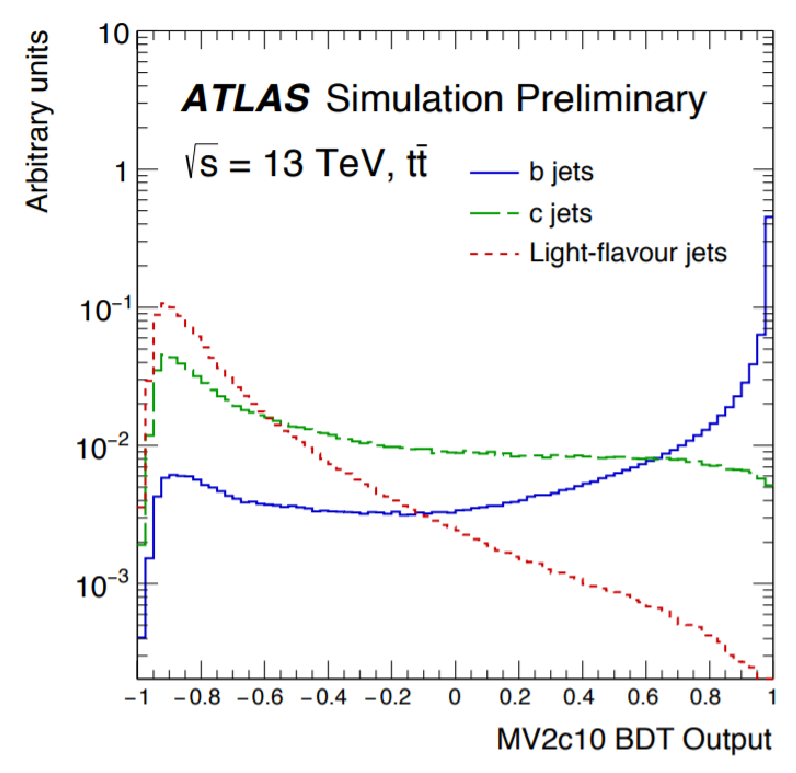
\includegraphics[width=0.54\linewidth]{MV2c10_output.eps}
    \caption{Output distribution of the MV2c10 algorithm for b-jets, charm jets, and light jets}
    \label{fig:MV2c10}
\end{figure}

From the output of the BDT, working points (WPs) are developed based on the efficiency of truth b-jets at particular values of the MV2c10 algorithm. The working points used in this analysis are summarized in table \ref{tab:btag_WPs}. 

\begin{table}[H]
\begin{center}
\begin{tabular}{|c|ccccc|}
    \hline
       WP &  none & loose & medium & tight & tightest\\
       \hline
     b eff. & - & 85\% & 77\% & 70\% & 60\% \\ 
    \hline
    \end{tabular}    
    \caption{B-tagging Working Points by tightness and b-jet efficiency}
    \label{tab:btag_WPs}
    \end{center}
\end{table}

A tighter WP will accept fewer b-jets, but reject a higher fraction of charm and light jets. Generally, analyses that include b-jets will use a fixed working point, for example, requiring that a jet pass the 70\% threshold. By instead treating these working point as bins, e.g. events with jets that fall between the 85\% and 77\% WPs fall into one bin, while events with jets passing the 60\% WP fall into another, and looking at the full psuedo-continuous MV2c10 spectrum of the jets, additional information can be gained. The psuedo-continuous b-tag spectrum is used in this case to separate out WZ + b, WZ + charm, and WZ + light. 

\subsection{Missing transverse energy}
\label{subsec:met}

Missing transverse momentum ($E_T^{miss}$) is used as part of the event selection. The missing transverse momentum vector is defined as the inverse of the sum of the transverse momenta of all reconstructed physics objects as well as remaining unclustered energy, the latter of which is estimated from low-\pt tracks associated with the primary vertex but not assigned to a hard object \cite{ATL-PHYS-PUB-2015-027}. 

%-------------------------------------------------------------------------------
\section{Event Selection}
\label{sec:evt_selection}
%-------------------------------------------------------------------------------

Selected events are required to include exactly three reconstructed light leptons passing the requirement described in \ref{subsec:leps}, which have a total charge of $\pm$1. As the opposite sign lepton is found to be prompt the vast majority of the time \cite{ttH_paper}, it is required to be loose and isolated, as defined though the standard \verb|isolationFixedCutLoose| working point supported by combined performance groups. The same sign leptons are required to be very tight, as per the recommended \verb|isolationFixedCutTight|.

The leptons are ordered in the analysis code as 0, 1, and 2. Lepton 0 is the lepton whose charge is opposite the other two. Lepton 1 is the lepton closest to the opposite charge lepton, i.e. the smallest $\Delta R$, leaving lepton 2 as the lepton further from the opposite charge lepton. Lepton 0 is required to have $p_T > 10$ GeV, while the same sign leptons, 1 and 2, are required to have $p_T > 20$ GeV to reduce the contribution of non-prompt leptons.  

The invariant mass of at least one pair of opposite sign, same flavor leptons is required to fall within 10 GeV of the mass of the Z boson, 91.2 GeV. Events where one of the opposite sign pairs have an invariant mass less than 12 GeV are rejected in order to suppress low mass resonances. %Further, events where the trilepton mass falls within 5 GeV of the Z mass are rejected to remove Z events that include conversions.

An additional requirement is placed on the missing transverse energy, $E^{miss}_T$ > 20 GeV, and the transverse mass of the $W$ candidate, $m(E^{miss}_T + l_{other}) > 30$ GeV, where $E^{miss}_T$ is the missing transverse energy, and $l_{other}$ is the lepton not included in the Z-candidate. 

Events are required to have one or two reconstructed jets passing the selection described in section \ref{subsec:jets}. Events with more than two jets are rejected in order to reduce the contribution of backgrounds such as $t\bar{t}Z$ and $t\bar{t}W$, which tend to have higher jet multiplicity. This selection of summarized in table \ref{tbl:selection}.

\begin{table}[h]
    \centering
    \begin{tabular}{l}
        \hline\hline
        Event Selection\\
        \hline 
        Exactly three leptons with charge $\pm$1 \\
        Two same-charge leptons with $p_T$ $>$ 20 GeV \\
        One opposite charge lepton with $p_T$ $>$ 10 GeV \\
        $m(l^+l^-)$ within 10 GeV of 91.2 GeV \\
        Transverse mass of W-candidate, $m_T(E_T^{miss} + lep_{other})$ $>$ 30 GeV \\
        Missing transverse energy, $E_T^{miss} >$ 20 GeV \\
        One or two jets with $p_T$ $>$ 25 GeV \\
        \hline\hline
    \end{tabular}
    \caption{Summary of the selection applied to events for inclusion in the fit}
    \label{tbl:selection}
\end{table}

%---------------------------
\subsection{Signal Region Validation}
\label{sec:SRkinematics}
%---------------------------

The event yields for both data and Monte Carlo are summarized in table \ref{tab:evt_yields}, which shows good agreement between data and Monte Carlo, and demonstrates that this signal region consists primarily of WZ events.

\begin{table}[H]
    \centering
        \begin{table}[htbp]
\begin{center}
\begin{tabular}{|c|c|}
\hline
Process & Events \\
\hline 
  $WZ + b$   & 143.5 \pm 3.3 \\ 
  $WZ + charm$   & 892.3 \pm 9.5 \\ 
  $WZ + light$   & 5952.6 \pm 26.9 \\ 
  Other $VV + b$   & 24.3 \pm 1.0 \\ 
  Other $VV + charm$   & 33.7 \pm 1.3 \\ 
  Other $VV + light$   & 487.4 \pm 5.8 \\ 
  $t\bar{t}W$   & 15.2 \pm 0.52 \\ 
  $t\bar{t}Z$   & 56.1 \pm 0.9 \\ 
  rare Top   & 3.8 \pm 0.2 \\ 
  $Z+\text{jets}$   & 301.7 \pm 27.1 \\ 
  $V+\gamma$   & 18.2 \pm 8.0 \\ 
  $tZ$   & 106.9 \pm 2.3 \\ 
  $tW$   & 8.7 \pm 2.4 \\ 
  $WtZ$   & 24.6 \pm 1.5 \\ 
  $VVV$   & 11.9 \pm 0.22 \\ 
  $VH$   & 21.7 \pm 4.5 \\ 
  $t\bar{t}$   & 320.9 \pm 12.3 \\ 
  $t\bar{t}H$   & 5.2 \pm 0.2 \\ 
\hline 
  Total  & 8435.66 \pm 42.93 \\ 
\hline
  Data   & 8640 \\
\hline 
\end{tabular} 
\caption{Events yields at 138.9 $fb^{-1}$} 
\end{center} 
\end{table} 

    \caption{Data and MC yields after the event selection requiring three leptons, one or two jets, $E^{miss}_T$ > 20 GeV, and $m(E^{miss}_T + l_{other}) > 30$ GeV has been applied.}
    \label{tab:evt_yields}
\end{table}

Here Other $VV$ represents diboson processes other than WZ, and consists predominantly of $ZZ\rightarrow llll$ events where one of the leptons is not reconstructed.

Simulations are further validated by comparing the kinematic distributions of the Monte Carlo with data, which are shown in figure \ref{sr_kinematics}.

%textbf{There is some discrepancies between data and MC, particularly in the low MET and low lepton $p_T$ regions, which are being investigated. This is suspected to be the result of underestimating the fake contribution, possibly because of several missing Z+jets simulation files.}

\begin{figure}[H]
    \subfigure[]{\includegraphics[width=0.47\textwidth]{kinematics/m3l.eps}}%
    %\begin{subfigure}{.48\textwidth}
    %    \includegraphics[width=1\linewidth]{kinematics/m3l.eps}
    %    \caption{}
    %    \label{fig:m3l}
    %\end{subfigure}%  
    \begin{subfigure}{.48\textwidth}
        \includegraphics[width=1\linewidth]{kinematics/HT.eps}
        \caption{}
        \label{fig:mll01}
    \end{subfigure}\\
    \begin{subfigure}{.48\textwidth}
        \includegraphics[width=1\linewidth]{kinematics/lead_jetPt.eps}
        \caption{}
        \label{fig:jetPt}
    \end{subfigure}%
    \begin{subfigure}{.48\textwidth}
        \includegraphics[width=1\linewidth]{kinematics/MET.eps}
        \caption{}
        \label{fig:met}
    \end{subfigure}\\
    \caption{Comparisons between the data and MC distributions in the signal region for (a) the invariant mass of the three leptons, (b) the $H_T$ of each event, (c) the $p_T$ of the leading jet, (d) the missing transverse energy.}    
\end{figure}
\begin{figure}[H]
    \begin{subfigure}{.48\textwidth}
        \includegraphics[width=1\linewidth]{kinematics/lep_Pt_0.eps}
        \caption{}
        \label{fig:lep_Pt_0}
    \end{subfigure}%
    \begin{subfigure}{.48\textwidth}
        \includegraphics[width=1\linewidth]{kinematics/lep_Pt_1.eps}
        \caption{}
        \label{fig:lep_Pt_1}
    \end{subfigure}\\
        \begin{subfigure}{.48\textwidth}
        \includegraphics[width=1\linewidth]{kinematics/lep_Pt_2.eps}
        \caption{}
        \label{fig:lep_Pt_2}
    \end{subfigure}%
    \begin{subfigure}{.48\textwidth}
        \includegraphics[width=1\linewidth]{kinematics/Mll01.eps}
        \caption{}
        \label{fig:Mll01}
    \end{subfigure}\\ 
    \caption{Comparisons between the data and MC distributions in the signal region for (a) the transverse momentum of the opposite sign lepton, (b) the transverse momentum of the same-sign lepton closest to the opposite sign lepton, (c) the $p_T$ of the lepton furthest from the opposite sign lepton, (d) the invariant mass of lepton 0 and lepton 1.}
\end{figure}
\begin{figure}[H]
    \begin{subfigure}{.48\textwidth}
        \includegraphics[width=1\linewidth]{kinematics/Mll02.eps}
        \caption{}
        \label{fig:Mll02}
    \end{subfigure}%
    \begin{subfigure}{.48\textwidth}
        \includegraphics[width=1\linewidth]{kinematics/Mll12.eps}
        \caption{}
        \label{fig:Mll12}
    \end{subfigure}\\
    \caption{Comparisons between the data and MC distributions in the signal region for (a) the invariant mass of leptons 0 and 2, (b) the invariant mass of the pair of leptons 1 and 2}
    \label{sr_kinematics}
\end{figure}

%---------------------------
\subsection{Non-Prompt Lepton Estimation}
\label{sec:fakes}
%---------------------------

Two processes act as sources of non-prompt leptons appear in the analysis: $t\bar{t}$ and $Z$+jet production both produce two prompt leptons, and each contribute to the signal region when an additional non-prompt lepton appears in the event. The contribution of these processes is estimated with Monte Carlo simulations, which are validated using enriched validation regions.

\subsubsection{$t\bar{t}$ Validation}

$t\bar{t}$ events can produce two prompt leptons from the decay of each of the tops. These top decays produce two b-quarks, the decay of which can produce additional non-prompt leptons, which occasionally pass the selection of the signal region. In order to validate that the Monte Carlo accurately simulates this process accurately, the MC prediction in a non-prompt $t\bar{t}$ enriched validation region is compared to data.

The $t\bar{t}$ validation region is similar to the signal region - three leptons meeting the criteria described in section \ref{sec:evt_selection} are required, and the requirements on $E_T^{miss}$ remain the same. However, the selection requiring a lepton pair form a Z-candidate are reversed. Events where the invariant mass of any two opposite sign, same flavor leptons falls within 10 GeV of 91.2 GeV are rejected. This ensures the $t\bar{t}$ validation region is orthogonal to the signal region. 

Further, because the jet multiplicity of $t\bar{t}$ events tends to be higher than WZ, the number of jets in each event is required to be greater than 1. As b-jets are almost invariably produced from top decays, at least one b-tagged jet in each event is required. 

%This selection creates a region which is dominated by $t\bar{t}$ events. The yields in this region are summarized in \ref{tab:ttbar_yields}.

%\begin{table}[H]
%    \centering
%        %\input{ttbar_yields.tex}
%    \caption{Data and MC yields after the event selection of the $t\bar{t}$ validation region has been applied.}
%    \label{tab:ttbar_yields}
%\end{table}

Various kinematic plots of this region are shown below. The general agreement between data and MC in each of these suggests that the non-prompt contribution of $t\bar{t}$ is well modeled by Monte Carlo.

\begin{figure}[H]
    \begin{subfigure}{.48\textwidth}
        \includegraphics[width=1\linewidth]{ttbar/m3l.eps}
        \caption{}
        \label{fig:ttbar_m3l}
    \end{subfigure}%  
    \begin{subfigure}{.48\textwidth}
        \includegraphics[width=1\linewidth]{ttbar/HT.eps}
        \caption{}
        \label{fig:ttbar_mll01}
    \end{subfigure}\\
    \begin{subfigure}{.48\textwidth}
        \includegraphics[width=1\linewidth]{ttbar/lead_jetPt.eps}
        \caption{}
        \label{fig:ttbar_jetPt}
    \end{subfigure}%
    \begin{subfigure}{.48\textwidth}
        \includegraphics[width=1\linewidth]{ttbar/MET.eps}
        \caption{}
        \label{fig:ttbar_met}
    \end{subfigure}\\
    \caption{Comparisons between the data and MC distributions in the $t\bar{t}$ validation region for (a) the invariant mass of the three leptons, (b) the $H_T$ of each event, (c) the $p_T$ of the leading jet, (d) the missing transverse energy.}    
    \end{figure}
\begin{figure}[H]
    \begin{subfigure}{.48\textwidth}
        \includegraphics[width=1\linewidth]{ttbar/lep_Pt_0.eps}
        \caption{}
        \label{fig:ttbar_lep_Pt_0}
    \end{subfigure}%
    \begin{subfigure}{.48\textwidth}
        \includegraphics[width=1\linewidth]{ttbar/lep_Pt_1.eps}
        \caption{}
        \label{fig:ttbar_lep_Pt_1}
    \end{subfigure}\\
        \begin{subfigure}{.48\textwidth}
        \includegraphics[width=1\linewidth]{ttbar/lep_Pt_2.eps}
        \caption{}
        \label{fig:ttbar_lep_Pt_2}
    \end{subfigure}%
    \begin{subfigure}{.48\textwidth}
        \includegraphics[width=1\linewidth]{ttbar/Mll01.eps}
        \caption{}
        \label{fig:ttbar_Mll01}
    \end{subfigure}\\ 
    \caption{Comparisons between the data and MC distributions in the $t\bar{t}$ validation region for (a) the transverse momentum of the opposite sign lepton, (b) the transverse momentum of the same-sign lepton closest to the opposite sign lepton, (c) the $p_T$ of the lepton furthest from the opposite sign lepton, (d) the invariant mass of lepton 0 and lepton 1.}
\end{figure}
\begin{figure}[H]
    \begin{subfigure}{.48\textwidth}
        \includegraphics[width=1\linewidth]{ttbar/nJets_OR_T.eps}
        \caption{}
        \label{fig:ttbar_nJets}
    \end{subfigure}%
    \begin{subfigure}{.48\textwidth}
        \includegraphics[width=1\linewidth]{ttbar/nJets_OR_T_MV2c10_70.eps}
        \caption{}
        \label{fig:ttbar_nbJets}
    \end{subfigure}\\
    \caption{Comparisons between the data and MC distributions in the $t\bar{t}$ validation region for (a) the number of jets, (b) the number of b-tagged jets.}
    \label{ttbar_kinematics}
\end{figure}

\subsubsection{$Z$+jets Validation}

Similar to $t\bar{t}$, a non-prompt $Z$+jets validation region is produced in order to validate the MC predictions. The lepton requirements remain the same as the signal region. Because no neutrinos are present for this process, the $E_T^{miss}$ cut is reversed, requiring $E_T^{miss}$ < 30 GeV. This also ensures this validation region is orthogonal to the signal region. Further, the number of jets in each event is required to be greater than one. 

Various kinematic plots of this region are shown below. The general agreement between data and MC in each of these suggests that the non-prompt contribution of $Z$+jets is well modeled by Monte Carlo.

\begin{figure}[H]
    \begin{subfigure}{.48\textwidth}
        \includegraphics[width=1\linewidth]{zjets/m3l.eps}
        \caption{}
        \label{fig:zjets_m3l}
    \end{subfigure}%  
    \begin{subfigure}{.48\textwidth}
        \includegraphics[width=1\linewidth]{zjets/HT.eps}
        \caption{}
        \label{fig:zjets_mll01}
    \end{subfigure}\\
    \begin{subfigure}{.48\textwidth}
        \includegraphics[width=1\linewidth]{zjets/lead_jetPt.eps}
        \caption{}
        \label{fig:zjets_jetPt}
    \end{subfigure}%
    \begin{subfigure}{.48\textwidth}
        \includegraphics[width=1\linewidth]{zjets/MET.eps}
        \caption{}
        \label{fig:zjets_met}
    \end{subfigure}\\
    \caption{Comparisons between the data and MC distributions in the $t\bar{t}$ validation region for (a) the invariant mass of the three leptons, (b) the $H_T$ of each event, (c) the $p_T$ of the leading jet, (d) the missing transverse energy.}    
    \end{figure}
\begin{figure}[H]
    \begin{subfigure}{.48\textwidth}
        \includegraphics[width=1\linewidth]{zjets/lep_Pt_0.eps}
        \caption{}
        \label{fig:zjets_lep_Pt_0}
    \end{subfigure}%
    \begin{subfigure}{.48\textwidth}
        \includegraphics[width=1\linewidth]{zjets/lep_Pt_1.eps}
        \caption{}
        \label{fig:zjets_lep_Pt_1}
    \end{subfigure}\\
        \begin{subfigure}{.48\textwidth}
        \includegraphics[width=1\linewidth]{zjets/lep_Pt_2.eps}
        \caption{}
        \label{fig:zjets_lep_Pt_2}
    \end{subfigure}%
    \begin{subfigure}{.48\textwidth}
        \includegraphics[width=1\linewidth]{zjets/Mll01.eps}
        \caption{}
        \label{fig:zjets_Mll01}
    \end{subfigure}\\ 
    \caption{Comparisons between the data and MC distributions in the $Z$+jets validation region for (a) the transverse momentum of the opposite sign lepton, (b) the transverse momentum of the same-sign lepton closest to the opposite sign lepton, (c) the $p_T$ of the lepton furthest from the opposite sign lepton, (d) the invariant mass of lepton 0 and lepton 1.}
\end{figure}
\begin{figure}[H]
    \begin{subfigure}{.48\textwidth}
        \includegraphics[width=1\linewidth]{zjets/nJets_OR_T.eps}
        \caption{}
        \label{fig:zjets_nJets}
    \end{subfigure}%
    \begin{subfigure}{.48\textwidth}
        \includegraphics[width=1\linewidth]{zjets/nJets_OR_T_MV2c10_70.eps}
        \caption{}
        \label{fig:zjets_nbJets}
    \end{subfigure}\\
    \caption{Comparisons between the data and MC distributions in the $Z$+jets validation region for (a) the number of jets, (b) the number of b-tagged jets.}
    \label{zjets_kinematics}
\end{figure}


%------------------------------------------------------------------------------- 
\section{tZ Interference Studies and Separation Multivariate Analysis}
\label{sec:tZ_bdt}
%------------------------------------------------------------------------------- 

Because it includes an on-shell Z boson as well as a b-jet and W from the top decay, tZ production represents an identical final state  to WZ + b-jet. This implies the possibility of matrix level interference between these two processes not accounted for in the Monte Carlo simulations, which consider the two processes independently. Truth level studies are performed in order to estimate the impact of these interference effects.

Because tZ produces a final state identical to signal, it represents a predominant background in the most signal enriched regions. Therefore, a boosted decision tree (BDT) algorithm is trained using TMVA \cite{TMVA_guide} to separate $WZ$ + heavy flavor from tZ.

Separation between tZ and $WZ$ + heavy flavor is achieved in part by reconstructing the invariant mass of the top candidate, which clusters more closely to the top mass for tZ than WZ + heavy flavor.

The result of this BDT is used to create a tZ enriched region in the fit, reducing its impact on the measurement of WZ + heavy flavor.

\subsection{Interference Studies}
\label{subsec:interference}

In order to estimate the matrix level interference effects between tZ and WZ + b-jet, two different sets of simulations are produced using MadGraph 5 \cite{Madgraph} - one which simulates these two processes independently, and another where they are produced simultaneously, such that interference effects are present. These two sets of samples are then compared, and the difference between them can be taken to represent any interference effects.

MadGraph simulations of 10,000 tZ and 10,000 WZ + b-jet events are produced, along with 20,000 events where both are present, in the fiducial region where 

The kinematics of these samples are shown below:



\subsection{Top Mass Reconstruction}
\label{subsec:topMass}

 The reconstruction of the top mass follows the procedure described in detail in section 6.1 of \cite{ttZ_paper}. The mass of the top quark candidate is reconstructed from the jet, the lepton not included in the Z-candidate, and a reconstructed neutrino. Since the selection requires exactly one jet in the event, there is only possible b-jet candidate. 

The neutrino from the W decay is expected to be the only source of $E_T^{miss}$. Therefore, the $E_T$ and $\phi$ of the neutrino are taken from the $E_T^{miss}$ measurement. This leaves the z-component of the neutrino momentum, $p_{\nu z}$ as the only unknown.

This unknown is solved for by taking the combined invariant mass of the lepton and neutrino to give the invariant mass of the $W$ boson:

\begin{center}
   $(p_l + p_{\nu})^2 = m_W^2$ \\ 
\end{center} 

Expanding this out into components, this equation gives:

\begin{center}
   $\sqrt{p_T_\nu^2+p_z_\nu^2}E_l = \frac{m^2_w-m^2_l}{2}+p_T_\nu(p_l_x cos\phi_\nu + p_l_y sin \phi_\nu) + p_l_z p_\nu_z$ \\ 
\end{center} 

This equation gives two solutions for $p_{\nu z}$. For cases where only one of these solutions is real, that is taken as the value of $p_{\nu z}$. For instances with two real solutions, the one which is shown to be correct in the largest fraction of simulations is taken. For cases when no real solution is found, often because of detector effects, the value of $E_T^{miss}$ is varied in decreasing increments of 100 MeV until a real solution is found.

The reconstructed top mass distribution for tZ and $WZ$ + b can be seen in figure \ref{fig:topMass}.

\begin{figure}
    \centering
    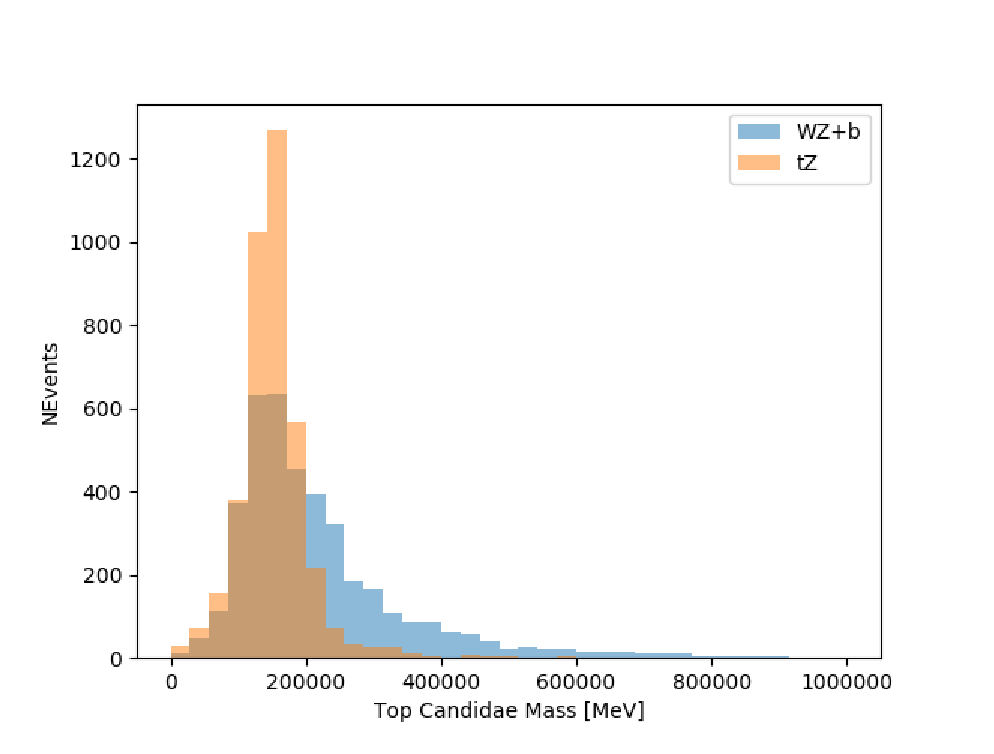
\includegraphics[width=0.7\linewidth]{tZ_bdt/topMass.eps}
    \caption{Reconstructed top mass distributions for tZ and $WZ$ + b, measured in MeV.}
    \label{fig:topMass}
\end{figure}

\subsection{tZ BDT}
\label{subsec:tZ_bdt}
 
The following kinematic variables are used as inputs in order to distinguish between these two processes:
 
 \begin{itemize}
     \item The invariant mass of the reconstructed top candidate
     \item $p_T$ of each of the leptons
     \item $E_T^{miss}$
     \item Distance between each combination of leptons, $\Delta R (ll)$
     \item Distance between each lepton and the jet, $\Delta R (lj)$
 \end{itemize}
 
The training samples included only events meeting the requirements of the 1-jet, >60\% region, i.e. passing all the selection described in section \ref{sec:evt_selection} and having exactly one jet which passes the tightest (60\%) MV2c10 working point. 
 
The distributions of these features for both signal and background is shown in figure \ref{fig:tZ_kinematics}.
 
\begin{figure}[H]
\center
    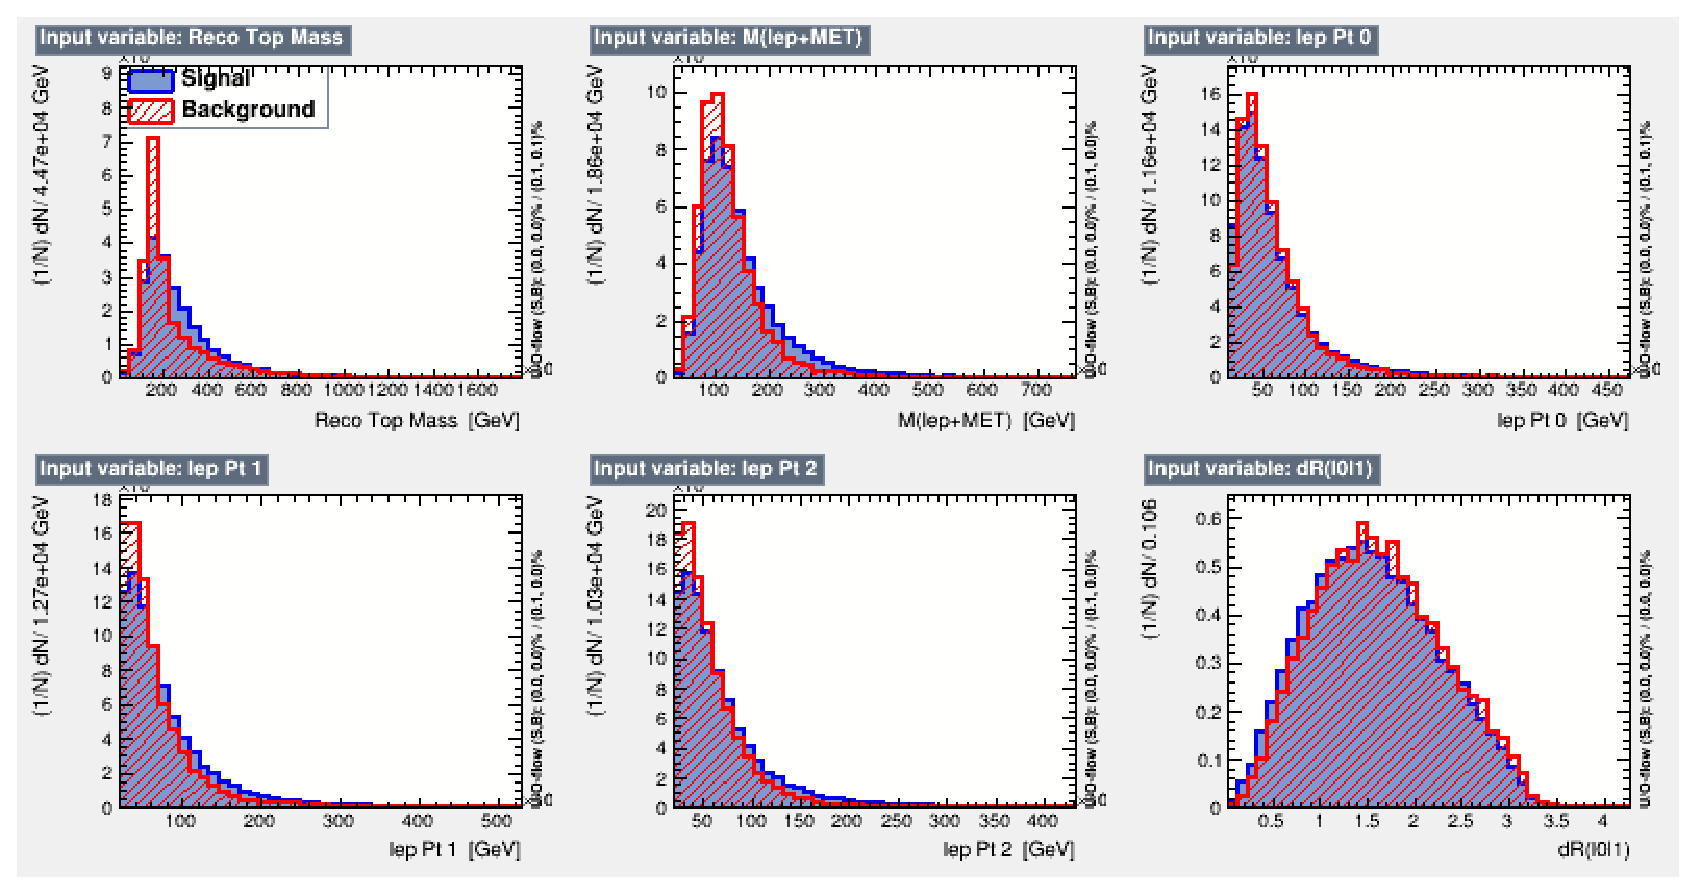
\includegraphics[width=0.9\linewidth]{tZ_bdt/variables_id_c1.eps}\\
    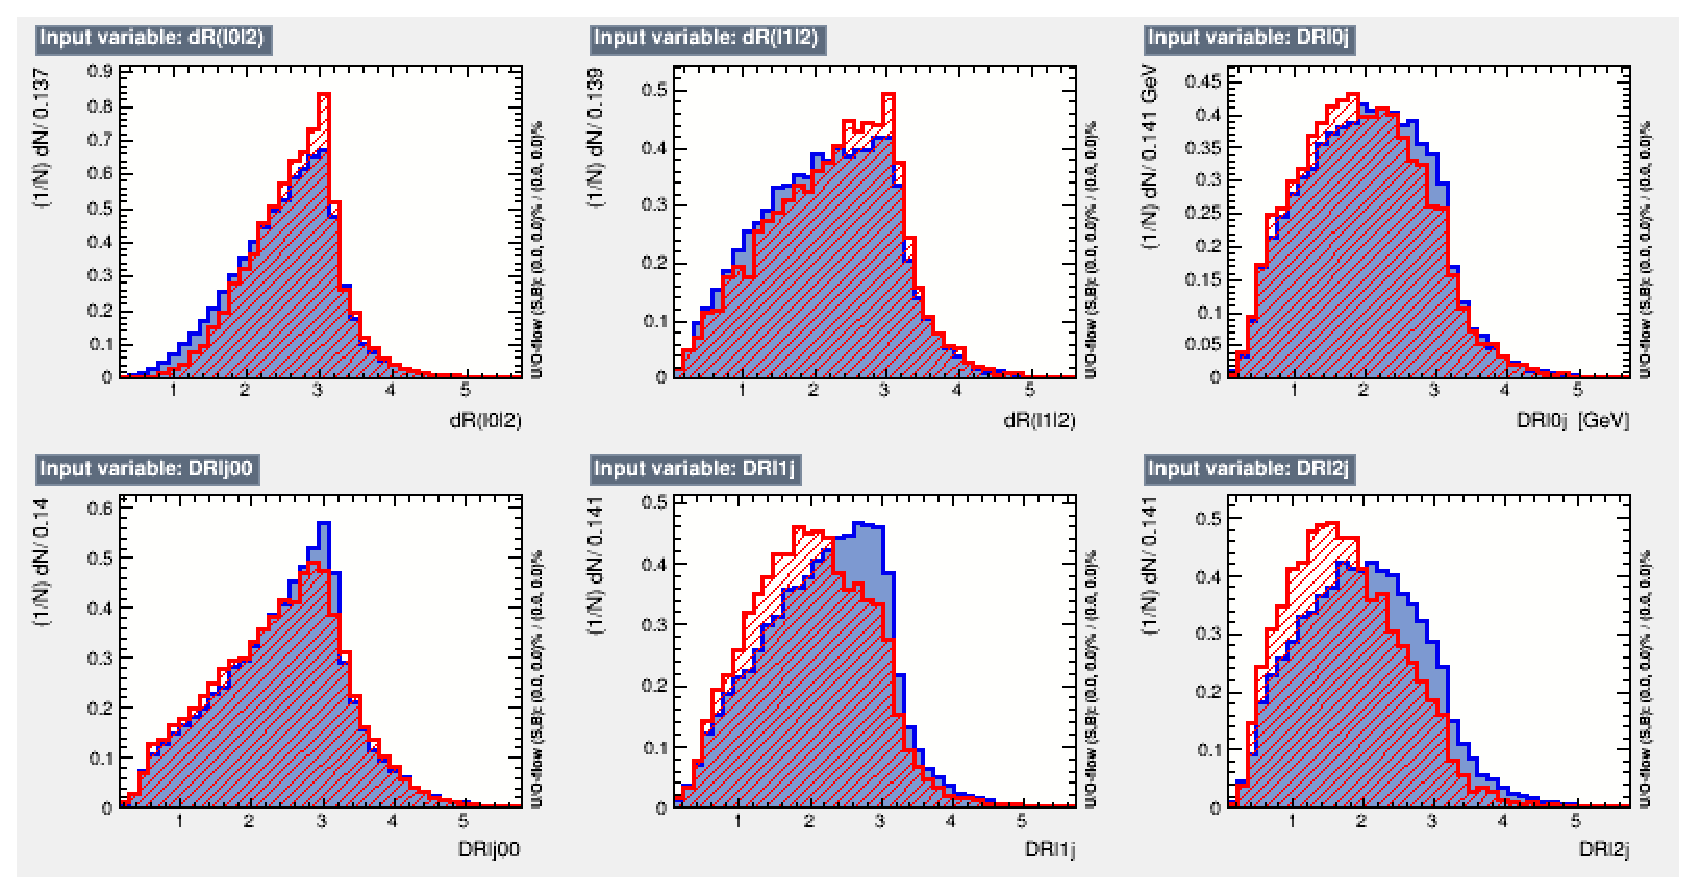
\includegraphics[width=0.9\linewidth]{tZ_bdt/variables_id_c2.eps}\\
    \caption{Distribution of input features of the BDT for signal (WZ) and background (tZ).}
    \label{fig:tZ_kinematics}
\end{figure}

A sample of 20,000 background (tZ) and signal (WZ+b) Monte Carlo events are used to train the BDT. And additional 5,000 events are reserved for testing the model, in order to prevent over-fitting. A total of 750 decision trees with a maximum depth of 6 branches are used to build the model. These parameters are chosen empirically, by training several models with different parameters and selecting the one that gave the best separation for the test sample. 

The results of the BDT training are shown in figure \ref{fig:tZ_bdt}. The output scores for both signal and background events is shown on the left. The right shows the receiving operating characteristic (ROC) curve that results from the MVA. The ROC curve represents the background rejection as a function of signal efficiency, where each point on the curve represents a different response score. The ROC curve of the BDT is compared to the performance of using an optimal set of flat selections on the same set of input variables.

\begin{figure}[H]
\center
    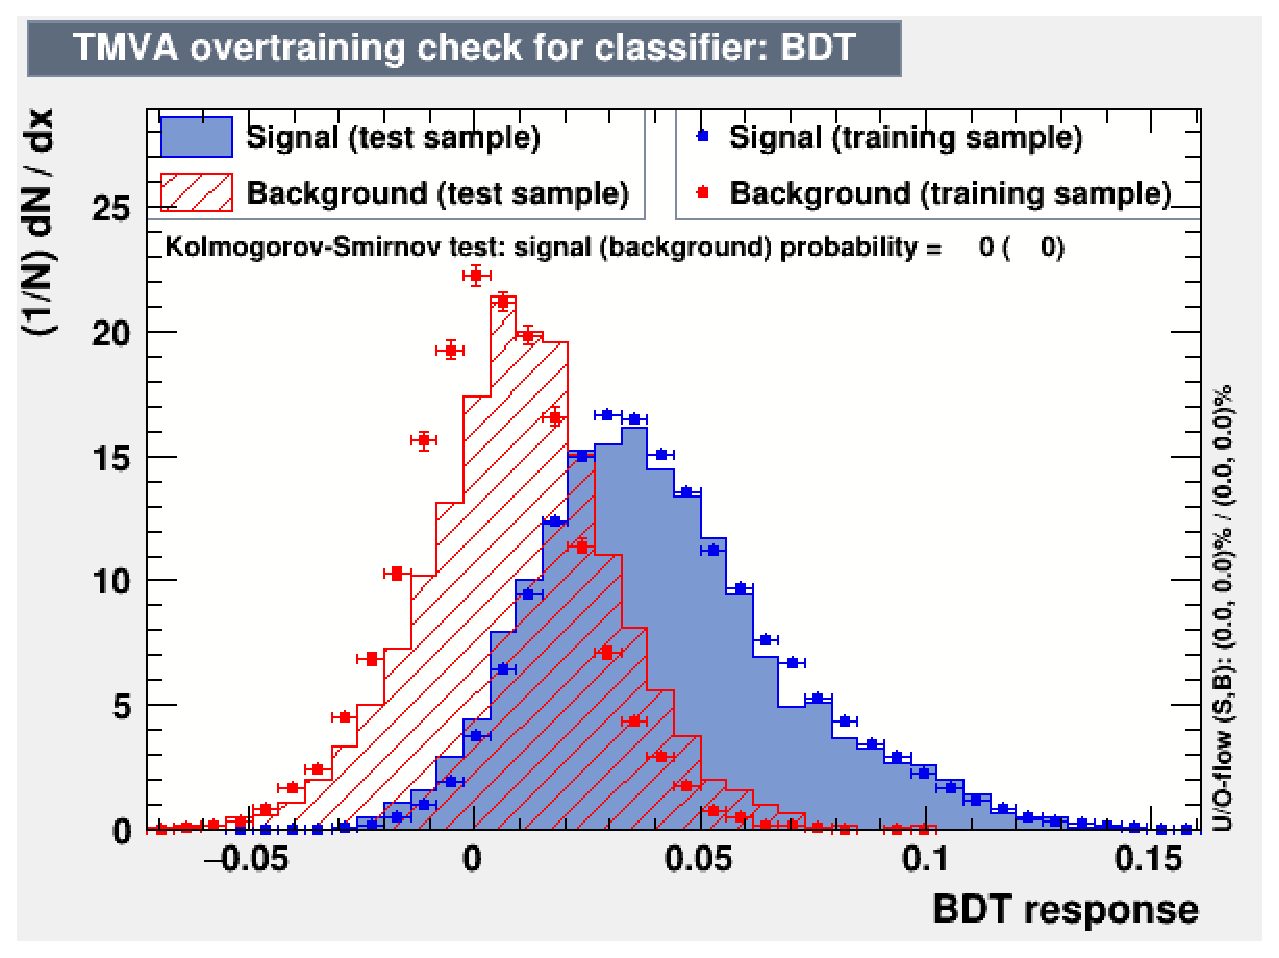
\includegraphics[width=.45\linewidth]{tZ_bdt/overtrain_BDT.eps}%                                     
    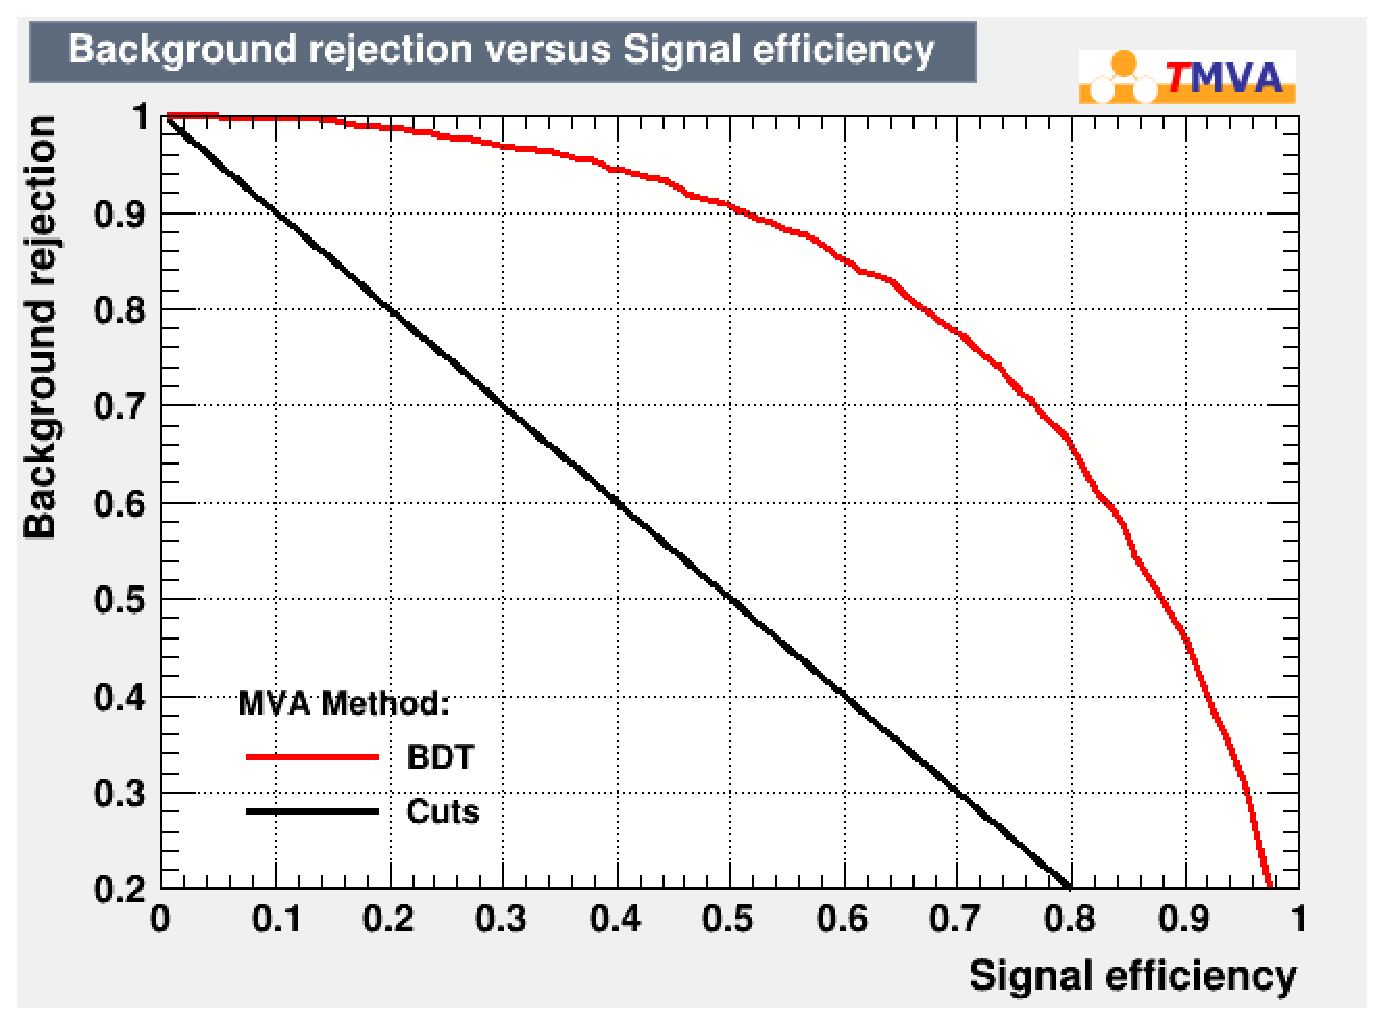
\includegraphics[width=.45\linewidth]{tZ_bdt/rejBvsS.eps}\\
    \caption{Distribution of the BDT response for signal and background events on the left, the ROC curve for the BDT on the right.}
    \label{fig:tZ_bdt}
\end{figure}

These results suggest that some amount of separation can be achieved between these two processes, with a high BDT score selecting a set of events that is pure in $WZ$ + b. Further, the ROC curve demonstrates the BDT performs significantly better than a flat selection.

%---------------------------------------------------------------------

\section{Signal Region Definitions}
\label{sec:signal_region}

The regions used in the fit are summarized in table \ref{tab:regions}.

\begin{table}[h]
\centering
\caption{A list of the regions used in the fit and the selection used for each.}
\begin{tabular}{l|l}
\hline\hline
Region & Selection  	      \\
\hline
\hline
1j, <85\%	& $N_{jets}$ = 1, jet MV2c10 < 85\%		      \\
1j, 85\%-77\%	& $N_{jets}$ = 1, 85\% < jet MV2c10 < 77\% 		      \\
1j, 77\%-70\%	& $N_{jets}$ = 1, 77\% < jet MV2c10 < 70\% 		      \\
1j, 70\%-60\%	& $N_{jets}$ = 1, 70\% < jet MV2c10 < 60\% 		      \\
1j, >60\%	& $N_{jets}$ = 1, jet MV2c10 > 85\%, tZ BDT score > 0.03 \\
tZ CR	& $N_{jets}$ = 1, jet MV2c10 > 85\% WP, tZ BDT score < 0.03 \\
2j, <85\%	& $N_{jets}$ = 2, jet MV2c10 score < 85\% WP		      \\
2j, 85\%-77\%	& $N_{jets}$ = 2, 85\% WP < jet MV2c10 score < 77\% WP		      \\
2j, 77\%-70\%	& $N_{jets}$ = 2, 77\% WP < jet MV2c10 score < 70\% WP		      \\
\hline\hline
\end{tabular}
\label{tab:regions}
\end{table}

The working points discussed in section \ref{subsec:bjets} are used to separate events into fit regions based on the highest working point reached by a jet in each event. Because the background composition differs significantly based on the number of b-jets, events are further subdivided into 1 jet and 2 jet regions in order to minimize the impact of background uncertainties. 

The two jet regions which fall within the tightest MV2c10 working points, between 70\%-60\% and 60\%, are left out of the fit. These regions are found to be dominated by leptonically decaying $t\bar{t}$ with an additional fake lepton. Because these regions add little statistical significance to the measurement while introducing large systematic uncertainties because of the prescence of a fake lepton, these regions are not included.

An additional tZ control region is created based on the BDT described in section \ref{sec:tZ_bdt}. The region with 1-jet passing the 60\% working point is split in two - a signal enriched region of events with a BDT score greater than 0.03, and a tZ control region including events with less than 0.03. This cutoff is arrived at by performing an Asimov fit with a variety of cutoffs, and selecting the value that produces the highest significance for the measurement of $WZ$ + b. 

%-------------------------------------------------------------------------------                                                                
%\section{Fitting Procedure}
%\label{sec:fit}
%-------------------------------------------------------------------------------                            



%-------------------------------------------------------------------------------

%-------------------------------------------------------------------------------
\section{Systematic Uncertainties}
\label{sec:sys}
%-------------------------------------------------------------------------------

The systematic uncertainties that are considered are summarized in table \ref{tab:systematics}. These are implemented in the fit either as a normalization factors or as a shape variation or both in the signal and background estimations. The numerical impact of each of these uncertainties is outlined in section \ref{sec:results}.

\begin{table}[h]
\centering
\caption{Sources of systematic uncertainty considered in the analysis.}
\begin{tabular}{lr}
\hline\hline
Systematic uncertainty & Components  	      \\
\hline
\hline
Luminosity	& 1		      \\
Pileup reweighting 	& 1		      \\
\textbf {Physics Objects}     	&		      \\
\ \ Electron                               	& 6		      \\
\ \ Muon	& 15		      \\
\ \ Jet energy scale and resolution  	& 28                  \\
\ \ Jet vertex fraction  	& 1		      \\
\ \ Jet flavor tagging   	& 131		      \\
\ \ $E^{miss}_T$  	& 3		      \\
\hline
Total (Experimental)        & 186		     \\
\hline
\hline
\textbf {Background Modeling}          	&		      \\
\ \ Cross section                 	& 24		      \\
\ \ Renormalization and factorization scales 	& 10		      \\
\ \ Parton shower and hadronization model       	& 2		      \\
\ \ Shower tune				& 4		      \\
\hline
Total (Signal and background modeling)       & 40		     \\
\hline\hline
Total (Overall)                             & 226	      \\
\hline\hline
\end{tabular}
\label{tab:SystSummary}
\end{table}

The uncertainty in the combined integrated luminosity is derived from a calibration of the luminosity scale performed in August 2015 and May 2016 \cite{lumi}.

The experimental uncertainties are related to the reconstruction and identification of light leptons and b-tagging of jets, and to the reconstruction of $E^{miss}_T$. The sources which contribute to the uncertainty in the jet energy scale \cite{jes} are decomposed into uncorrelated components and treated as independent sources in the analysis. 

The uncertainties in the b-tagging efficiencies measured in dedicated calibration analyses \cite{btag_cal} are also decomposed into uncorrelated components. The large number of components for b-tagging is due to the calibration of the distribution of the BDT discriminant.  

The systematic uncertainties associated with the signal and background processes are accounted for by varying the cross-section of each process within its uncertainty.

The full list of systematic uncertainties considered in the analysis is summarized in tables
\ref{Tab:LeptonExperimentalSyst}, \ref{Tab:JetsExperimentalSyst} and \ref{Tab:BTagExperimentalSyst}.

\hspace{-1in}\begin{table}[H]
  \begin{center}
    {\small
    \begin{tabular}{|llcl|}
      \hline
      \multicolumn{4}{|c|}{\bf Experimental Systematics on Leptons and $E_T^{miss}$} \\
     % \hline
      Type     & Description  & Systematics Name & Application \\
     \hline
     \hline
     \multicolumn{4}{|c|}{\bf{Trigger}}\\
     \hline
    Scale Factors    & Trigger Efficiency        & lepSFTrigTight$\_$MU(EL)$\_$SF$\_$Trigger$\_$STAT(SYST)    & Event Weight      \\
      \hline
      \multicolumn{4}{|c|}{\bf{Muons}} \\
      \hline
      Efficiencies   & Reconstruction and        & lepSFObjTight$\_$MU$\_$SF$\_$ID$\_$STAT(SYST)              & Event Weight       \\
     & Identification    &       &        \\
      & Isolation                 &       lepSFObjTight$\_$MU$\_$SF$\_$Isol$\_$STAT(SYST)            & Event Weight       \\
         & Track To Vertex   	 & lepSFObjTight$\_$MU$\_$SF$\_$TTVA$\_$STAT(SYST )           & Event Weight       \\
    & Association  		 &   							      &           \\
     \pt Scale   & \pt Scale & MUONS$\_$SCALE    & \pt Correction     \\
     &   &   &           \\
      Resolution     & Inner Detector            & MUONS$\_$ID        					      & \pt Correction     \\
         & Energy Resolution      	 &     &         \\
    & Muon Spectrometer    	 & MUONS$\_$MS      & \pt Correction     \\
     & Energy Resolution         &       &        \\
     &   &   &         \\
     \hline
     \multicolumn{4}{|c|}{\bf{Electrons}}\\
     \hline
     Efficiencies    & Reconstruction       	 & lepSFObjTight$\_$EL$\_$SF$\_$ID  			      & Event Weight   	    \\
     & Identification   & lepSFObjTight$\_$EL$\_$SF$\_$Reco       		      & Event Weight            \\
        & Isolation                 & lepSFObjTight$\_$EL$\_$SF$\_$Isol      		      & Event Weight        \\
       &   &   &          \\
     Scale Factor    & Energy  Scale             & EG$\_$SCALE$\_$ALL  					      & Energy Correction    \\
         	     &   &   &          \\
     Resolution      & Energy Resolution  	 & EG$\_$RESOLUTION$\_$ALL      			      & Energy Correction     \\
         	     &   &   &             \\
     \hline
     \multicolumn{4}{|c|}{\bf{$E_T^{miss}$}}\\
     \hline
     Soft Tracks Terms         &             Resolution                   &      MET$\_$SoftTrk$\_$ResoPerp       &   \pt Correction  \\
                               &             Resolution                   &      MET$\_$SoftTrk$\_$ResoPara        &    \pt Correction    \\
                               &             Scale                        &      MET$\_$SoftTrk$\_$ScaleUp         &   \pt Correction     \\
                               &             Scale                        &      MET$\_$SoftTrk$\_$ScaleDown         &   \pt Correction     \\

     \hline
     
    \end{tabular}
   }
   \caption{\label{Tab:LeptonExperimentalSyst} Summary of experimental systematics considered for leptons and $E_T^{miss}$. Includes type, description, name of systematic as used in the fit, and mode of application. The mode of application indicates the systematic evaluation, e.g. as an  overall event re-weighting (Event Weight) or rescaling (\pt Correction).}
  \end{center}
\end{table}


\begin{table}[H]
  \begin{center}
    {\small
    \begin{tabular}{|llcc|}
      \hline
      \multicolumn{4}{|c|}{\bf Experimental Systematics on Jets} \\
      \hline
      Type     & Origin   & Systematics Name  & Application \\
      \hline
      Jet Vertex Tagger         &     & JVT      &        Event Weight          \\
     	&   &   &     \\
      Energy Scale              & Calibration Method              & JET$\_$21NP$\_$           &      \pt Correction         \\
       &   & JET$\_$EffectiveNP$\_$1-19     &    \pt Correction  \\
       &   &   &       \\
        & $\eta$ inter-calibration        & JET$\_$EtaIntercalibration$\_$Modelling    & \pt Correction          \\
     &                                 & JET$\_$EtaIntercalibration$\_$NonClosure   & \pt Correction      \\
     &                                 & JET$\_$EtaIntercalibration$\_$TotalStat    & \pt Correction      \\
    &   &   &        \\
     & High \pt jets                   & JET$\_$SingleParticle$\_$HighPt         &     \pt Correction             \\
     	&   &   &           \\
        & Pile-Up                         & JET$\_$Pileup$\_$OffsetNPV            &     \pt Correction             \\
        &       & JET$\_$Pileup$\_$OffsetMu             &     \pt Correction               \\
        &        & JET$\_$Pileup$\_$PtTerm       &     \pt Correction         \\
        &                                         & JET$\_$Pileup$\_$RhoTopology      &     \pt Correction             \\
    	&   &   &            \\
          & Non Closure                     & JET$\_$PunchThrough$\_$MC15    & \pt Correction    \\
    	&   &   &       \\
         & Flavour                         & JET$\_$Flavor$\_$Response          &   \pt Correction            \\
     &         & JET$\_$BJES$\_$Response          &   \pt Correction           \\
           &                                 & JET$\_$Flavor$\_$Composition        &    \pt Correction             \\
         	&   &   &          \\
      Resolution         	&                                 & JET$\_$JER$\_$SINGLE$\_$NP          &  Event Weight       \\
        			&   &   &          \\
        			
    \hline

     \end{tabular}
    }
    \caption{\label{Tab:JetsExperimentalSyst} Jet systematics take into account effects of jets calibration method, $\eta$ inter-calibration, high \pt jets, pile-up, and flavor response. They are all diagonalised into effective parameters.}
 \end{center}
\end{table}

\begin{table}[H]
  \begin{center}
    {\small
    \begin{tabular}{|llc|}
      \hline
     \multicolumn{3}{|c|}{\bf Experimental Systematics on b-tagging} \\
      \hline
      Type     & Origin   & Systematic Name \\
     \hline
     &   &                \\
      Scale Factors & MV2c10 b-tagger efficiency & MC2c10$\_$Continuous$\_$EventWeight$\_$B0-29 \\
      &    on b originated jets in bins of $\eta$  &   \\
      &   &                \\
      &    MC2c10 b-tagger efficiency & MC2c10$\_$Continuous$\_$EventWeight$\_$C0-19  \\
      &    on c originated jets in bins of $\eta$    &     \\
      &   &   \\
      &    MC2c10 b-tagger efficiency & MC2c10$\_$Continuous$\_$EventWeight$\_$Light0-79           \\
      &    on light flavoured originated jets         &   \\
     &     in bins of $\eta$ and \pt      &    \\
         &   &             \\
     &    MC2c10 b-tagger                        & MC2c10$\_$Continuous$\_$EventWeight$\_$extrapolation  \\
     &    extrapolation efficiency    &         MC2c10$\_$Continuous$\_$EventWeight$\_$extrapolation$\_$from$\_$charm             \\
     \hline
    \end{tabular}
    }
    \caption{\label{Tab:BTagExperimentalSyst} Summary of experimental systematics to be included for $b$-tagging of jets in the analysis, using the continuous MC2c10 tagging algorithm. All of the b-tagging related systematics are applied as event weights. From left: type, description, and the name of systematic used in the fit.}
  \end{center}
\end{table}

%--------------------------------------
                                                                
\section{Results}
\label{sec:results}
%-------------------------------------------------------------------------------    

A maximum-likelihood fit is performed simultaneously over these nine regions in order to extract the best-fit value of the WZ + b-jet and WZ + charm jet contributions. The $WZ$ + b, $WZ$ + charm and $WZ$ + light contributions are allowed to float, with the remaining background contributions are held fixed. \textbf{The current fit strategy treats the WZ + b-jet contribution as the parameter of interest, with the normalization of the $WZ$ + charm and the $WZ$ + light contributions taken as systematic uncertainties. This could however be adjusted, depending on whether it is decided the goal of the analysis should be to measure WZ+b specifically or WZ + heavy flavor overall.} The result of the fit is used to extract the cross-section of $WZ$ + heavy-flavor production.

A maximum likelihood fit to data is performed simultaneously in the eight regions described in section \ref{sec:signal_region}. The parameters $\mu_{WZ+b}$, $\mu_{WZ+charm}$, $\mu_{WZ+light}$, where $\mu = \sigma_{observed}/\sigma_{SM} $, are extracted from the fit.

%The fit gives a $\mu$ value of $1.3^{+0.5}_{-0.4}(stat)^{+0.4}_{-0.4}(sys)$ for $WZ$ + b. The fitted cross-section modifiers for $WZ$ + charm and $WZ$ + light are $1.2 \pm 0.2 \pm 0.1$ and $1.04 \pm 0.04 \pm 0.03 $, respectively, consistent with Standard Model predictions. The observed $WZ$ + heavy-flavor inclusive cross-section is $124^{+51}_{-43}(stat)^{+36}_{-35}(sys)$ fb = $124^{+63}_{-56}$ fb. This is calculated based on a model dependant extrapolation to an inclusive region of phase space. 
\textbf{The results of the fit are currently blinded.} The post-fit yields in each region are summarized in figure \ref{fig:fit_regions}.

\begin{figure}
    \center
    \includegraphics[width=.35\linewidth]{all_b/not_85_postFit.eps}%                                     
    \includegraphics[width=.35\linewidth]{all_b/WP_1b_77_85_postFit.eps}%
    \includegraphics[width=.35\linewidth]{all_b/WP_1b_70_77_postFit.eps}\\
    \includegraphics[width=.35\linewidth]{all_b/WP_1b_60_70_postFit.eps}%                                     
    \includegraphics[width=.35\linewidth]{all_b/WP_1b_60_postFit.eps}%
    \includegraphics[width=.35\linewidth]{all_b/tZ_CR_postFit.eps}\\
    \includegraphics[width=.35\linewidth]{all_b/WP_2b_77_85_postFit.eps}%                                     
    \includegraphics[width=.35\linewidth]{all_b/WP_2b_70_77_postFit.eps}\\
    \caption{Data/MC results in each of the regions after the fit has been performed.}
    \label{fig:fit_regions}
\end{figure}

A post-fit summary plot of the fitted regions is shown in figure \ref{fig:fit_results}: 

\begin{figure}[H]
    \center
    \includegraphics[width=.9\linewidth]{all_b/Summary_postFit.eps}
    \caption{Post-fit summary of fit.}
    \label{fig:fit_results}
\end{figure}

As described in section \ref{sec:sys}, there are 226 systematic uncertainties that are considered as NPs in the fit. These NPs are constrained by Gaussian or log-normal probability density functions. The latter are used for normalisation factors to ensure that they are always positive. The expected numbers
of signal and background events are functions of the likelihood. The prior for each NP is added as a penalty term, decreasing the likelihood as it is shifted away from its nominal value. 

The impact of each systematic uncertainty is calculated by performing the fit with the parameter of interest held fixed, varied from its fitted value by its uncertainty, and calculating $\delta\mu$ relative to the baseline fit.  The impact of the most significant systematic uncertainties is summarized in table \ref{tab:systematics}. 

\begin{table}[H]
    \centering
    \begin{tabular}{l|cc}
        \hline\hline
        Uncertainty Source & \multicolumn{2}{c}{$\Delta \mu$ }  \\
        \hline
        WZ + charm cross-section & -0.1966 & 0.2171 \\
        tZ cross-section & -0.1521 & 0.1518 \\
        WZ + light cross-section & 0.1485 & -0.1411 \\
        Other VV + b cross-sction & -0.1115 & 0.1163 \\
        Flavor Tagging & 0.0955 & 0.0957 \\
        Jet Energy Scale & 0.0613 & 0.081 \\
        $t\bar{t}$ cross-section & -0.0662 & 0.0654 \\
        Luminosity & -0.0609 & 0.0655 \\
        Z + jets cross-section & -0.0284 & 0.0284 \\
        Other VV + charm cross-sction & 0.0207 & -0.0202 \\
        Muon Trigger Scale Factor & 0.019 & 0.0209 \\
        \hline
        Total Systematic Uncertainty & 0.3511 & 0.3679 \\
        \hline\hline
    \end{tabular}
    \caption{Summary of the most significant sources of systematic uncertainty.}
    \label{tab:systematics}
\end{table}

The ranking and impact of those nuisance parameters with the largest contribution to the overall uncertainty is shown in figure \ref{fig:ranking}.

\begin{figure}[H]
    \centering
    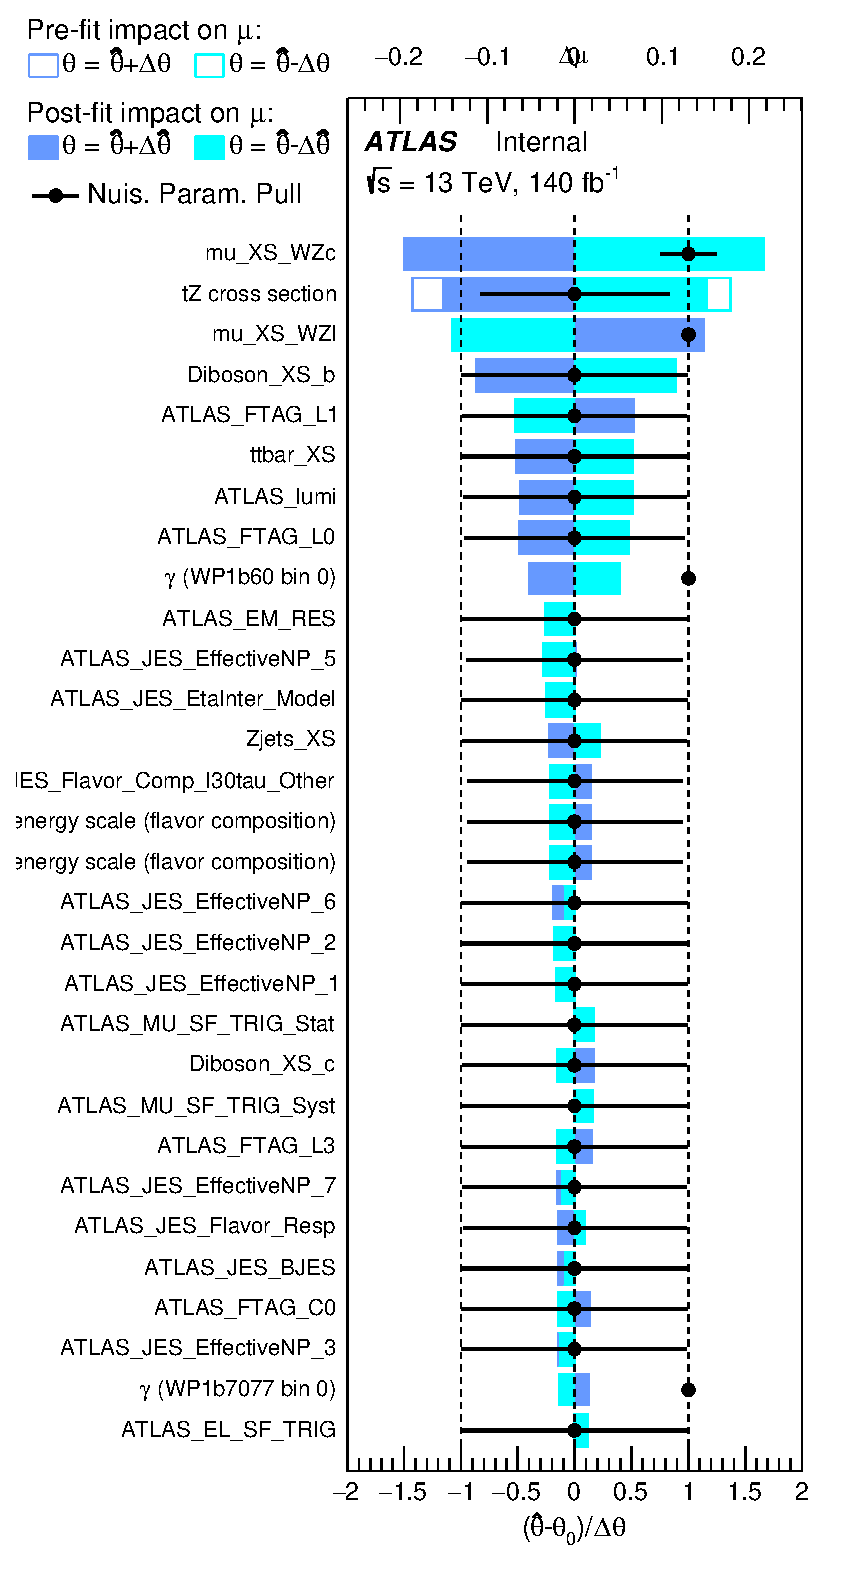
\includegraphics[width=0.7\linewidth]{all_b/Ranking.eps}
    \caption{Impact of systematic uncertainties on the signal-strength of $WZ$ + b}
    \label{fig:ranking}
\end{figure}

The large impact of the Jet Energy Scale and Jet Flavor Tagging is unsurprising, as the shape of the fit regions depends heavily on the modeling of the jets. The other major sources of uncertainty come from background modelling and cross-section uncertainty. The pie charts in figure \ref{fig:pie_chart} show that for the modelling uncertainties that contribute most correspond to the most significant backgrounds. %The pileup-reweighting and luminosity play a significant role as well, because, as shown in figure \ref{fig:pie_chart}, the signal purity is relatively small in each of the fit regions. This means that a small scaling in the background contribution resulting from a change in luminosity or pileup corresponds to a significant change in the best fit signal contribution. 

\begin{figure}[H]
    \centering
    \includegraphics[width=0.7\linewidth]{all_b/PieChart_postFit.eps}
    \caption{Background composition of the fit regions.}
    \label{fig:pie_chart}
\end{figure}

The correlations between these nuisance parameters are summarized in figure \ref{fig:corr_mat}. 

\begin{figure}[H]
    \centering
    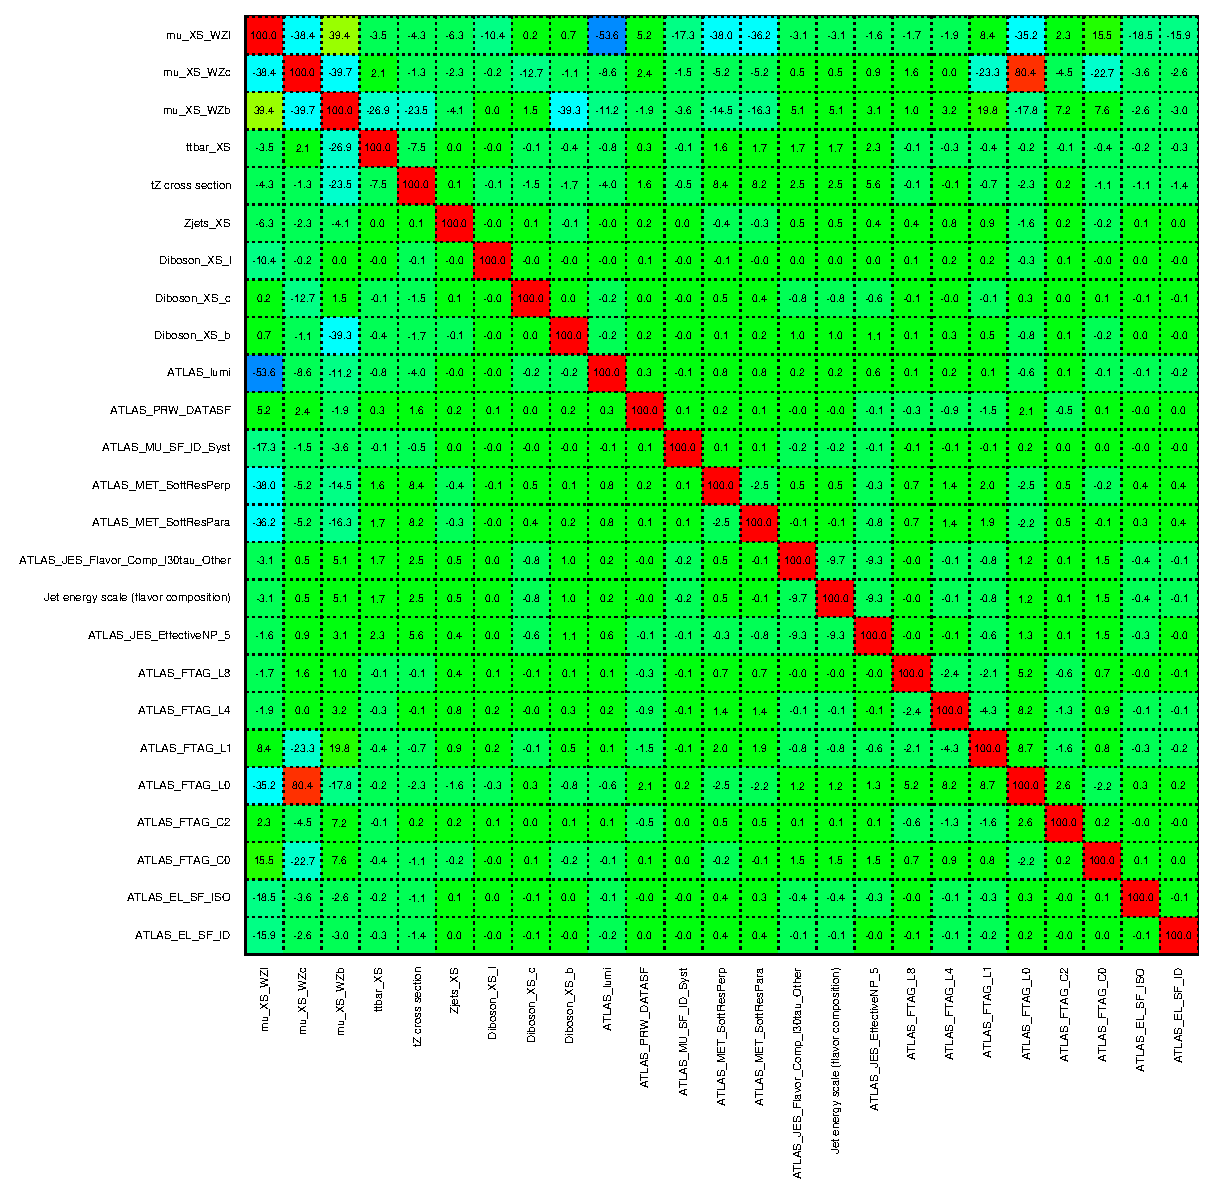
\includegraphics[width=1.0\linewidth]{all_b/CorrMatrix.eps}
    \caption{Correlations between nuisance parameters}
    \label{fig:corr_mat}
\end{figure}

The negative correlations between $\mu_{WZ+charm}$ and $\mu_{WZ+b}$ and $\mu_{WZ+light}$ are expected: $WZ$ + charm is present in both the $WZ$ + b and $WZ$ + light enriched regions, therefore increasing the fraction of charm requires increasing the fraction of $WZ$ + b and $WZ$ + light. This reasoning also explains the positive correlation between $\mu_{WZ+b}$ and $\mu_{WZ+light}$. 

Two of the major backgrounds in the region with the highest purity of $WZ$ + b are tZ and Other VV + b, explaining the negative correlations between $\mu_{WZ+b}$ and the tZ cross section, and the VV + b cross section.

The high correlation between the luminosity and $\mu_{WZ+light}$ arises from the fact that the uncertainty on $\mu_{WZ+light}$ is very low (around 4\%). Small changes in luminosity cause a change in the yield of $WZ$ + light that is large compared to its uncertainty, producing a large correlation between these two parameters.

%The other significant correlation present is between ATLAS FTAG L0 and $\mu_{WZ + light}$ and $\mu_{WZ+ charm}$. This shifts the   

%\begin{figure}[H]
%    \centering
%    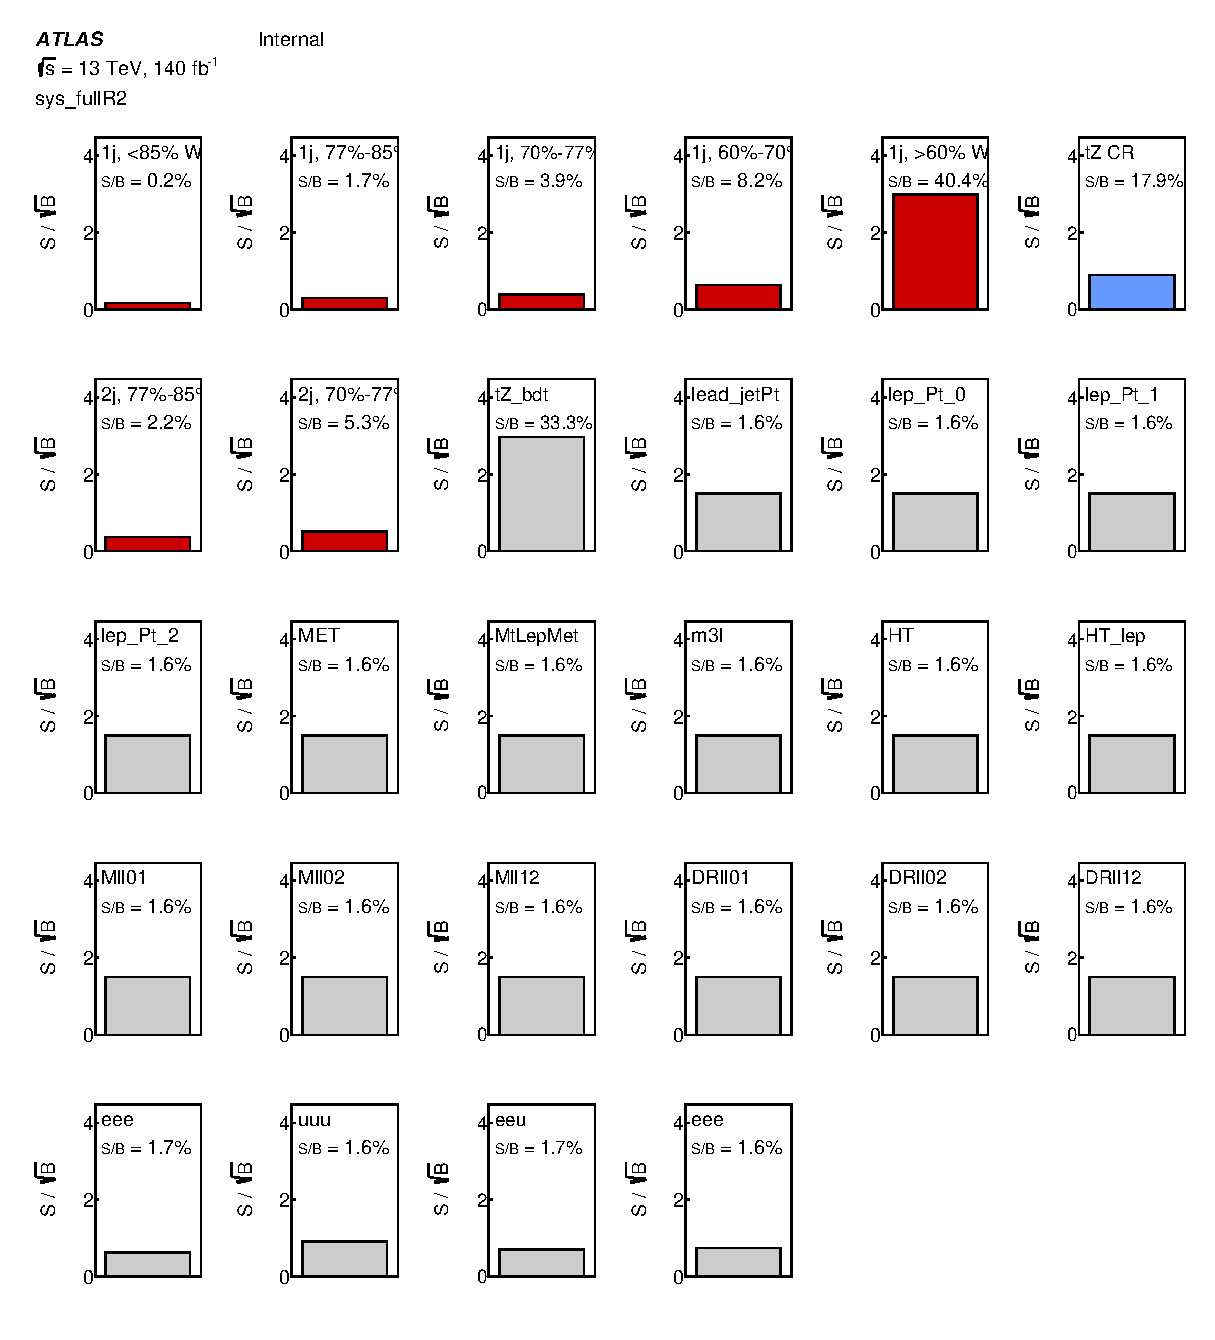
\includegraphics[width=0.63\linewidth]{all_b/SignalRegions.eps}
%    \caption{Significance, given by $S/\sqrt{B}$ of the signal in each of the fit regions.}
%    \label{fig:signalRegions}
%\end{figure}

%\newpage
%\begin{landscape}
%\begin{table}[htbp]
%\begin{center}
%\caption{\label{tbl:yields} Background, signal and observed yields in the twelve analysis categories in 36.1 %\ifb\ of data at $\sqrt{s} =$ 13~TeV. Uncertainties in the background estimates due to systematic effects and %t.}
% \resizebox{1.3\textwidth}{!}{
%        \begin{tabular}{|c|c|c|c|c|c|c|c|c|c|}
\hline 
 & $<$85 WP & 1b, 77-85 WP & 1b, 70-77 WP & 1b, 60-70 WP & 1b, $>$60 WP & 2b, 77-85 WP & 2b, 70-77 WP & 2b, 60-70 WP & 2b, $>$60 WP\\
\hline 
  $t\bar{t}W$   & \num[round-mode=figures,round-precision=3]{2.27655} $\pm$ \num[round-mode=figures,round-precision=3]{2.30791} & \num[round-mode=figures,round-precision=3]{1.3571} $\pm$ \num[round-mode=figures,round-precision=3]{1.35835} & \num[round-mode=figures,round-precision=3]{0.941663} $\pm$ \num[round-mode=figures,round-precision=3]{0.969334} & \num[round-mode=figures,round-precision=3]{1.99269} $\pm$ \num[round-mode=figures,round-precision=3]{1.98343} & \num[round-mode=figures,round-precision=3]{10.3804} $\pm$ \num[round-mode=figures,round-precision=3]{10.3282} & \num[round-mode=figures,round-precision=3]{1.50549} $\pm$ \num[round-mode=figures,round-precision=3]{1.50488} & \num[round-mode=figures,round-precision=3]{1.16646} $\pm$ \num[round-mode=figures,round-precision=3]{1.16209} & \num[round-mode=figures,round-precision=3]{1.37188} $\pm$ \num[round-mode=figures,round-precision=3]{1.36002} & \num[round-mode=figures,round-precision=3]{3.85472} $\pm$ \num[round-mode=figures,round-precision=3]{3.818} \\ 
  $t\bar{t}Z$   & \num[round-mode=figures,round-precision=3]{5.59481} $\pm$ \num[round-mode=figures,round-precision=3]{0.952561} & \num[round-mode=figures,round-precision=3]{1.85638} $\pm$ \num[round-mode=figures,round-precision=3]{0.457615} & \num[round-mode=figures,round-precision=3]{1.61823} $\pm$ \num[round-mode=figures,round-precision=3]{0.288506} & \num[round-mode=figures,round-precision=3]{2.22864} $\pm$ \num[round-mode=figures,round-precision=3]{0.409013} & \num[round-mode=figures,round-precision=3]{14.0042} $\pm$ \num[round-mode=figures,round-precision=3]{3.50867} & \num[round-mode=figures,round-precision=3]{1.86738} $\pm$ \num[round-mode=figures,round-precision=3]{0.362445} & \num[round-mode=figures,round-precision=3]{1.14193} $\pm$ \num[round-mode=figures,round-precision=3]{0.396228} & \num[round-mode=figures,round-precision=3]{1.15182} $\pm$ \num[round-mode=figures,round-precision=3]{0.425086} & \num[round-mode=figures,round-precision=3]{2.7131} $\pm$ \num[round-mode=figures,round-precision=3]{0.684245} \\ 
  $VV + b$   & \num[round-mode=figures,round-precision=3]{9.26027} $\pm$ \num[round-mode=figures,round-precision=3]{5.07692} & \num[round-mode=figures,round-precision=3]{5.31041} $\pm$ \num[round-mode=figures,round-precision=3]{2.6598} & \num[round-mode=figures,round-precision=3]{5.63769} $\pm$ \num[round-mode=figures,round-precision=3]{3.04505} & \num[round-mode=figures,round-precision=3]{4.7021} $\pm$ \num[round-mode=figures,round-precision=3]{2.56084} & \num[round-mode=figures,round-precision=3]{30.7357} $\pm$ \num[round-mode=figures,round-precision=3]{14.5166} & \num[round-mode=figures,round-precision=3]{1.89107} $\pm$ \num[round-mode=figures,round-precision=3]{1.01403} & \num[round-mode=figures,round-precision=3]{1.02904} $\pm$ \num[round-mode=figures,round-precision=3]{0.505366} & \num[round-mode=figures,round-precision=3]{1.37878} $\pm$ \num[round-mode=figures,round-precision=3]{0.681346} & \num[round-mode=figures,round-precision=3]{1.23094} $\pm$ \num[round-mode=figures,round-precision=3]{0.856462} \\ 
  $VV + c$   & \num[round-mode=figures,round-precision=3]{228.417} $\pm$ \num[round-mode=figures,round-precision=3]{51.3311} & \num[round-mode=figures,round-precision=3]{62.547} $\pm$ \num[round-mode=figures,round-precision=3]{13.4738} & \num[round-mode=figures,round-precision=3]{31.8} $\pm$ \num[round-mode=figures,round-precision=3]{7.84773} & \num[round-mode=figures,round-precision=3]{23.5735} $\pm$ \num[round-mode=figures,round-precision=3]{5.96178} & \num[round-mode=figures,round-precision=3]{23.9244} $\pm$ \num[round-mode=figures,round-precision=3]{6.99115} & \num[round-mode=figures,round-precision=3]{4.56139} $\pm$ \num[round-mode=figures,round-precision=3]{1.46901} & \num[round-mode=figures,round-precision=3]{1.23133} $\pm$ \num[round-mode=figures,round-precision=3]{1.07988} & \num[round-mode=figures,round-precision=3]{0.116983} $\pm$ \num[round-mode=figures,round-precision=3]{0.164252} & \num[round-mode=figures,round-precision=3]{--} $\pm$ \num[round-mode=figures,round-precision=3]{--} \\ 
  $VV + l$   & \num[round-mode=figures,round-precision=3]{2240.34} $\pm$ \num[round-mode=figures,round-precision=3]{85.2546} & \num[round-mode=figures,round-precision=3]{114.763} $\pm$ \num[round-mode=figures,round-precision=3]{11.1222} & \num[round-mode=figures,round-precision=3]{31.8071} $\pm$ \num[round-mode=figures,round-precision=3]{5.36505} & \num[round-mode=figures,round-precision=3]{16.8257} $\pm$ \num[round-mode=figures,round-precision=3]{3.80662} & \num[round-mode=figures,round-precision=3]{6.47758} $\pm$ \num[round-mode=figures,round-precision=3]{2.25164} & \num[round-mode=figures,round-precision=3]{2.36682} $\pm$ \num[round-mode=figures,round-precision=3]{1.23121} & \num[round-mode=figures,round-precision=3]{0.357081} $\pm$ \num[round-mode=figures,round-precision=3]{0.365519} & \num[round-mode=figures,round-precision=3]{0.0167576} $\pm$ \num[round-mode=figures,round-precision=3]{0.0232322} & \num[round-mode=figures,round-precision=3]{--} $\pm$ \num[round-mode=figures,round-precision=3]{--} \\ 
  $t\bar{t}$   & \num[round-mode=figures,round-precision=3]{27.761} $\pm$ \num[round-mode=figures,round-precision=3]{357.388} & \num[round-mode=figures,round-precision=3]{--} $\pm$ \num[round-mode=figures,round-precision=3]{--} & \num[round-mode=figures,round-precision=3]{--} $\pm$ \num[round-mode=figures,round-precision=3]{--} & \num[round-mode=figures,round-precision=3]{0.000302665} $\pm$ \num[round-mode=figures,round-precision=3]{2.1126e-05} & \num[round-mode=figures,round-precision=3]{36.0985} $\pm$ \num[round-mode=figures,round-precision=3]{407.045} & \num[round-mode=figures,round-precision=3]{0.000302665} $\pm$ \num[round-mode=figures,round-precision=3]{2.1126e-05} & \num[round-mode=figures,round-precision=3]{0.000302665} $\pm$ \num[round-mode=figures,round-precision=3]{2.1126e-05} & \num[round-mode=figures,round-precision=3]{0.000302665} $\pm$ \num[round-mode=figures,round-precision=3]{2.1126e-05} & \num[round-mode=figures,round-precision=3]{0.48602} $\pm$ \num[round-mode=figures,round-precision=3]{1.7566} \\ 
  $t\bar{t}+\gamma$   & \num[round-mode=figures,round-precision=3]{0.480558} $\pm$ \num[round-mode=figures,round-precision=3]{1.05386} & \num[round-mode=figures,round-precision=3]{0.000320031} $\pm$ \num[round-mode=figures,round-precision=3]{0.000152476} & \num[round-mode=figures,round-precision=3]{0.197334} $\pm$ \num[round-mode=figures,round-precision=3]{1.00686} & \num[round-mode=figures,round-precision=3]{0.209157} $\pm$ \num[round-mode=figures,round-precision=3]{1.06389} & \num[round-mode=figures,round-precision=3]{0.887418} $\pm$ \num[round-mode=figures,round-precision=3]{2.72954} & \num[round-mode=figures,round-precision=3]{0.492239} $\pm$ \num[round-mode=figures,round-precision=3]{2.48655} & \num[round-mode=figures,round-precision=3]{0.000320031} $\pm$ \num[round-mode=figures,round-precision=3]{0.000152476} & \num[round-mode=figures,round-precision=3]{0.000320031} $\pm$ \num[round-mode=figures,round-precision=3]{0.000152476} & \num[round-mode=figures,round-precision=3]{0.241039} $\pm$ \num[round-mode=figures,round-precision=3]{1.23072} \\ 
  Single top t-chan   & \num[round-mode=figures,round-precision=3]{0.000302869} $\pm$ \num[round-mode=figures,round-precision=3]{1.86387e-05} & \num[round-mode=figures,round-precision=3]{0.000302869} $\pm$ \num[round-mode=figures,round-precision=3]{1.86387e-05} & \num[round-mode=figures,round-precision=3]{0.000302869} $\pm$ \num[round-mode=figures,round-precision=3]{1.86387e-05} & \num[round-mode=figures,round-precision=3]{0.000302869} $\pm$ \num[round-mode=figures,round-precision=3]{1.86387e-05} & \num[round-mode=figures,round-precision=3]{0.000302869} $\pm$ \num[round-mode=figures,round-precision=3]{1.86387e-05} & \num[round-mode=figures,round-precision=3]{0.000302869} $\pm$ \num[round-mode=figures,round-precision=3]{1.86387e-05} & \num[round-mode=figures,round-precision=3]{0.000302869} $\pm$ \num[round-mode=figures,round-precision=3]{1.86387e-05} & \num[round-mode=figures,round-precision=3]{0.000302869} $\pm$ \num[round-mode=figures,round-precision=3]{1.86387e-05} & \num[round-mode=figures,round-precision=3]{0.000302869} $\pm$ \num[round-mode=figures,round-precision=3]{1.86387e-05} \\ 
  Single top s-chan   & \num[round-mode=figures,round-precision=3]{0.000302869} $\pm$ \num[round-mode=figures,round-precision=3]{1.86387e-05} & \num[round-mode=figures,round-precision=3]{0.000302869} $\pm$ \num[round-mode=figures,round-precision=3]{1.86387e-05} & \num[round-mode=figures,round-precision=3]{0.000302869} $\pm$ \num[round-mode=figures,round-precision=3]{1.86387e-05} & \num[round-mode=figures,round-precision=3]{0.000302869} $\pm$ \num[round-mode=figures,round-precision=3]{1.86387e-05} & \num[round-mode=figures,round-precision=3]{0.000302869} $\pm$ \num[round-mode=figures,round-precision=3]{1.86387e-05} & \num[round-mode=figures,round-precision=3]{0.000302869} $\pm$ \num[round-mode=figures,round-precision=3]{1.86387e-05} & \num[round-mode=figures,round-precision=3]{0.000302869} $\pm$ \num[round-mode=figures,round-precision=3]{1.86387e-05} & \num[round-mode=figures,round-precision=3]{0.000302869} $\pm$ \num[round-mode=figures,round-precision=3]{1.86387e-05} & \num[round-mode=figures,round-precision=3]{0.000302869} $\pm$ \num[round-mode=figures,round-precision=3]{1.86387e-05} \\ 
  $Wt$   & \num[round-mode=figures,round-precision=3]{0.362598} $\pm$ \num[round-mode=figures,round-precision=3]{0.654777} & \num[round-mode=figures,round-precision=3]{0.000302787} $\pm$ \num[round-mode=figures,round-precision=3]{1.86339e-05} & \num[round-mode=figures,round-precision=3]{0.108486} $\pm$ \num[round-mode=figures,round-precision=3]{0.584642} & \num[round-mode=figures,round-precision=3]{0.000302787} $\pm$ \num[round-mode=figures,round-precision=3]{1.86339e-05} & \num[round-mode=figures,round-precision=3]{0.274423} $\pm$ \num[round-mode=figures,round-precision=3]{0.503357} & \num[round-mode=figures,round-precision=3]{0.000302787} $\pm$ \num[round-mode=figures,round-precision=3]{1.86339e-05} & \num[round-mode=figures,round-precision=3]{0.000302787} $\pm$ \num[round-mode=figures,round-precision=3]{1.86339e-05} & \num[round-mode=figures,round-precision=3]{0.000302787} $\pm$ \num[round-mode=figures,round-precision=3]{1.86339e-05} & \num[round-mode=figures,round-precision=3]{0.000302787} $\pm$ \num[round-mode=figures,round-precision=3]{1.86339e-05} \\ 
  Three top   & \num[round-mode=figures,round-precision=3]{0.0003606} $\pm$ \num[round-mode=figures,round-precision=3]{0.0017759} & \num[round-mode=figures,round-precision=3]{0.000302946} $\pm$ \num[round-mode=figures,round-precision=3]{0.000150851} & \num[round-mode=figures,round-precision=3]{0.000302946} $\pm$ \num[round-mode=figures,round-precision=3]{0.000150851} & \num[round-mode=figures,round-precision=3]{0.000302946} $\pm$ \num[round-mode=figures,round-precision=3]{0.000150851} & \num[round-mode=figures,round-precision=3]{0.000612547} $\pm$ \num[round-mode=figures,round-precision=3]{0.00110042} & \num[round-mode=figures,round-precision=3]{0.000302946} $\pm$ \num[round-mode=figures,round-precision=3]{0.000150851} & \num[round-mode=figures,round-precision=3]{0.000302946} $\pm$ \num[round-mode=figures,round-precision=3]{0.000150851} & \num[round-mode=figures,round-precision=3]{0.000302946} $\pm$ \num[round-mode=figures,round-precision=3]{0.000150851} & \num[round-mode=figures,round-precision=3]{0.000773585} $\pm$ \num[round-mode=figures,round-precision=3]{0.00117832} \\ 
  Four top   & \num[round-mode=figures,round-precision=3]{0.000302952} $\pm$ \num[round-mode=figures,round-precision=3]{0.000150853} & \num[round-mode=figures,round-precision=3]{0.000302952} $\pm$ \num[round-mode=figures,round-precision=3]{0.000150853} & \num[round-mode=figures,round-precision=3]{0.000302952} $\pm$ \num[round-mode=figures,round-precision=3]{0.000150853} & \num[round-mode=figures,round-precision=3]{0.000302952} $\pm$ \num[round-mode=figures,round-precision=3]{0.000150853} & \num[round-mode=figures,round-precision=3]{0.000302952} $\pm$ \num[round-mode=figures,round-precision=3]{0.000150853} & \num[round-mode=figures,round-precision=3]{0.000302952} $\pm$ \num[round-mode=figures,round-precision=3]{0.000150853} & \num[round-mode=figures,round-precision=3]{0.000302952} $\pm$ \num[round-mode=figures,round-precision=3]{0.000150853} & \num[round-mode=figures,round-precision=3]{0.000302952} $\pm$ \num[round-mode=figures,round-precision=3]{0.000150853} & \num[round-mode=figures,round-precision=3]{0.00126998} $\pm$ \num[round-mode=figures,round-precision=3]{0.00683589} \\ 
  $t\bar{t}WW$   & \num[round-mode=figures,round-precision=3]{0.00022652} $\pm$ \num[round-mode=figures,round-precision=3]{0.00351054} & \num[round-mode=figures,round-precision=3]{0.000302883} $\pm$ \num[round-mode=figures,round-precision=3]{3.64287e-05} & \num[round-mode=figures,round-precision=3]{0.00440409} $\pm$ \num[round-mode=figures,round-precision=3]{0.0238607} & \num[round-mode=figures,round-precision=3]{0.0129946} $\pm$ \num[round-mode=figures,round-precision=3]{0.0319054} & \num[round-mode=figures,round-precision=3]{0.0062717} $\pm$ \num[round-mode=figures,round-precision=3]{0.0322067} & \num[round-mode=figures,round-precision=3]{0.00440409} $\pm$ \num[round-mode=figures,round-precision=3]{0.0238607} & \num[round-mode=figures,round-precision=3]{0.000302883} $\pm$ \num[round-mode=figures,round-precision=3]{3.64287e-05} & \num[round-mode=figures,round-precision=3]{0.000302883} $\pm$ \num[round-mode=figures,round-precision=3]{3.64287e-05} & \num[round-mode=figures,round-precision=3]{0.00571661} $\pm$ \num[round-mode=figures,round-precision=3]{0.0304709} \\ 
  $V+\text{jets}$   & \num[round-mode=figures,round-precision=3]{15.2819} $\pm$ \num[round-mode=figures,round-precision=3]{20.5512} & \num[round-mode=figures,round-precision=3]{0.373017} $\pm$ \num[round-mode=figures,round-precision=3]{0.281037} & \num[round-mode=figures,round-precision=3]{0.334766} $\pm$ \num[round-mode=figures,round-precision=3]{0.214858} & \num[round-mode=figures,round-precision=3]{0.364992} $\pm$ \num[round-mode=figures,round-precision=3]{0.306013} & \num[round-mode=figures,round-precision=3]{2.61101} $\pm$ \num[round-mode=figures,round-precision=3]{1.33608} & \num[round-mode=figures,round-precision=3]{0.141037} $\pm$ \num[round-mode=figures,round-precision=3]{0.202839} & \num[round-mode=figures,round-precision=3]{0.000291241} $\pm$ \num[round-mode=figures,round-precision=3]{0.000116691} & \num[round-mode=figures,round-precision=3]{0.000291241} $\pm$ \num[round-mode=figures,round-precision=3]{0.000116691} & \num[round-mode=figures,round-precision=3]{0.0279002} $\pm$ \num[round-mode=figures,round-precision=3]{0.152993} \\ 
  low mass $V+\text{jets}$   & \num[round-mode=figures,round-precision=3]{0.000291241} $\pm$ \num[round-mode=figures,round-precision=3]{0.000116691} & \num[round-mode=figures,round-precision=3]{0.000291241} $\pm$ \num[round-mode=figures,round-precision=3]{0.000116691} & \num[round-mode=figures,round-precision=3]{0.000291241} $\pm$ \num[round-mode=figures,round-precision=3]{0.000116691} & \num[round-mode=figures,round-precision=3]{0.000291241} $\pm$ \num[round-mode=figures,round-precision=3]{0.000116691} & \num[round-mode=figures,round-precision=3]{0.000291241} $\pm$ \num[round-mode=figures,round-precision=3]{0.000116691} & \num[round-mode=figures,round-precision=3]{0.000291241} $\pm$ \num[round-mode=figures,round-precision=3]{0.000116691} & \num[round-mode=figures,round-precision=3]{0.000291241} $\pm$ \num[round-mode=figures,round-precision=3]{0.000116691} & \num[round-mode=figures,round-precision=3]{0.000291241} $\pm$ \num[round-mode=figures,round-precision=3]{0.000116691} & \num[round-mode=figures,round-precision=3]{0.000291241} $\pm$ \num[round-mode=figures,round-precision=3]{0.000116691} \\ 
  $V+\text{jets}$   & \num[round-mode=figures,round-precision=3]{0.000302868} $\pm$ \num[round-mode=figures,round-precision=3]{1.10053e-05} & \num[round-mode=figures,round-precision=3]{0.000302868} $\pm$ \num[round-mode=figures,round-precision=3]{1.10053e-05} & \num[round-mode=figures,round-precision=3]{0.000302868} $\pm$ \num[round-mode=figures,round-precision=3]{1.10053e-05} & \num[round-mode=figures,round-precision=3]{0.000302868} $\pm$ \num[round-mode=figures,round-precision=3]{1.10053e-05} & \num[round-mode=figures,round-precision=3]{0.000302868} $\pm$ \num[round-mode=figures,round-precision=3]{1.10053e-05} & \num[round-mode=figures,round-precision=3]{0.000302868} $\pm$ \num[round-mode=figures,round-precision=3]{1.10053e-05} & \num[round-mode=figures,round-precision=3]{0.000302868} $\pm$ \num[round-mode=figures,round-precision=3]{1.10053e-05} & \num[round-mode=figures,round-precision=3]{0.000302868} $\pm$ \num[round-mode=figures,round-precision=3]{1.10053e-05} & \num[round-mode=figures,round-precision=3]{0.000302868} $\pm$ \num[round-mode=figures,round-precision=3]{1.10053e-05} \\ 
  $V+\gamma$   & \num[round-mode=figures,round-precision=3]{40.5736} $\pm$ \num[round-mode=figures,round-precision=3]{14.4393} & \num[round-mode=figures,round-precision=3]{1.10864} $\pm$ \num[round-mode=figures,round-precision=3]{0.529551} & \num[round-mode=figures,round-precision=3]{1.45353} $\pm$ \num[round-mode=figures,round-precision=3]{0.889563} & \num[round-mode=figures,round-precision=3]{0.112777} $\pm$ \num[round-mode=figures,round-precision=3]{0.585685} & \num[round-mode=figures,round-precision=3]{0.356533} $\pm$ \num[round-mode=figures,round-precision=3]{0.273389} & \num[round-mode=figures,round-precision=3]{0.000302868} $\pm$ \num[round-mode=figures,round-precision=3]{1.10053e-05} & \num[round-mode=figures,round-precision=3]{0.000302868} $\pm$ \num[round-mode=figures,round-precision=3]{1.10053e-05} & \num[round-mode=figures,round-precision=3]{0.000302868} $\pm$ \num[round-mode=figures,round-precision=3]{1.10053e-05} & \num[round-mode=figures,round-precision=3]{0.000302868} $\pm$ \num[round-mode=figures,round-precision=3]{1.10053e-05} \\ 
  $tZ$   & \num[round-mode=figures,round-precision=3]{11.5641} $\pm$ \num[round-mode=figures,round-precision=3]{1.10741} & \num[round-mode=figures,round-precision=3]{3.83557} $\pm$ \num[round-mode=figures,round-precision=3]{0.344865} & \num[round-mode=figures,round-precision=3]{3.22506} $\pm$ \num[round-mode=figures,round-precision=3]{0.290839} & \num[round-mode=figures,round-precision=3]{4.41135} $\pm$ \num[round-mode=figures,round-precision=3]{0.403135} & \num[round-mode=figures,round-precision=3]{27.7444} $\pm$ \num[round-mode=figures,round-precision=3]{2.48965} & \num[round-mode=figures,round-precision=3]{1.56275} $\pm$ \num[round-mode=figures,round-precision=3]{0.159151} & \num[round-mode=figures,round-precision=3]{0.745832} $\pm$ \num[round-mode=figures,round-precision=3]{0.0819564} & \num[round-mode=figures,round-precision=3]{0.665967} $\pm$ \num[round-mode=figures,round-precision=3]{0.0689025} & \num[round-mode=figures,round-precision=3]{1.31404} $\pm$ \num[round-mode=figures,round-precision=3]{0.136992} \\ 
  $WtZ$   & \num[round-mode=figures,round-precision=3]{3.34641} $\pm$ \num[round-mode=figures,round-precision=3]{1.63649} & \num[round-mode=figures,round-precision=3]{1.01967} $\pm$ \num[round-mode=figures,round-precision=3]{0.532459} & \num[round-mode=figures,round-precision=3]{0.912386} $\pm$ \num[round-mode=figures,round-precision=3]{0.464022} & \num[round-mode=figures,round-precision=3]{0.7321} $\pm$ \num[round-mode=figures,round-precision=3]{0.373417} & \num[round-mode=figures,round-precision=3]{4.21335} $\pm$ \num[round-mode=figures,round-precision=3]{2.05616} & \num[round-mode=figures,round-precision=3]{0.458102} $\pm$ \num[round-mode=figures,round-precision=3]{0.246527} & \num[round-mode=figures,round-precision=3]{0.221432} $\pm$ \num[round-mode=figures,round-precision=3]{0.13283} & \num[round-mode=figures,round-precision=3]{0.248025} $\pm$ \num[round-mode=figures,round-precision=3]{0.138019} & \num[round-mode=figures,round-precision=3]{0.162435} $\pm$ \num[round-mode=figures,round-precision=3]{0.100658} \\ 
  $VVV$   & \num[round-mode=figures,round-precision=3]{6.22694} $\pm$ \num[round-mode=figures,round-precision=3]{3.09521} & \num[round-mode=figures,round-precision=3]{0.473923} $\pm$ \num[round-mode=figures,round-precision=3]{0.254746} & \num[round-mode=figures,round-precision=3]{0.10713} $\pm$ \num[round-mode=figures,round-precision=3]{0.0617345} & \num[round-mode=figures,round-precision=3]{0.117184} $\pm$ \num[round-mode=figures,round-precision=3]{0.065154} & \num[round-mode=figures,round-precision=3]{0.0592735} $\pm$ \num[round-mode=figures,round-precision=3]{0.03952} & \num[round-mode=figures,round-precision=3]{0.0291393} $\pm$ \num[round-mode=figures,round-precision=3]{0.0270894} & \num[round-mode=figures,round-precision=3]{0.00323562} $\pm$ \num[round-mode=figures,round-precision=3]{0.00432544} & \num[round-mode=figures,round-precision=3]{0.00030518} $\pm$ \num[round-mode=figures,round-precision=3]{0.000151427} & \num[round-mode=figures,round-precision=3]{0.00030518} $\pm$ \num[round-mode=figures,round-precision=3]{0.000151427} \\ 
  $VH$   & \num[round-mode=figures,round-precision=3]{23.9715} $\pm$ \num[round-mode=figures,round-precision=3]{6.0978} & \num[round-mode=figures,round-precision=3]{0.852682} $\pm$ \num[round-mode=figures,round-precision=3]{1.3381} & \num[round-mode=figures,round-precision=3]{0.309145} $\pm$ \num[round-mode=figures,round-precision=3]{1.5312} & \num[round-mode=figures,round-precision=3]{0.764878} $\pm$ \num[round-mode=figures,round-precision=3]{2.34321} & \num[round-mode=figures,round-precision=3]{0.000302868} $\pm$ \num[round-mode=figures,round-precision=3]{1.10053e-05} & \num[round-mode=figures,round-precision=3]{0.000302868} $\pm$ \num[round-mode=figures,round-precision=3]{1.10053e-05} & \num[round-mode=figures,round-precision=3]{0.000302868} $\pm$ \num[round-mode=figures,round-precision=3]{1.10053e-05} & \num[round-mode=figures,round-precision=3]{0.000302868} $\pm$ \num[round-mode=figures,round-precision=3]{1.10053e-05} & \num[round-mode=figures,round-precision=3]{0.000302868} $\pm$ \num[round-mode=figures,round-precision=3]{1.10053e-05} \\ 
  $tHjb$   & \num[round-mode=figures,round-precision=3]{0.0419189} $\pm$ \num[round-mode=figures,round-precision=3]{0.0144183} & \num[round-mode=figures,round-precision=3]{0.0093033} $\pm$ \num[round-mode=figures,round-precision=3]{0.00855833} & \num[round-mode=figures,round-precision=3]{0.000302911} $\pm$ \num[round-mode=figures,round-precision=3]{3.57751e-05} & \num[round-mode=figures,round-precision=3]{0.00324645} $\pm$ \num[round-mode=figures,round-precision=3]{0.00803724} & \num[round-mode=figures,round-precision=3]{0.0372004} $\pm$ \num[round-mode=figures,round-precision=3]{0.0112587} & \num[round-mode=figures,round-precision=3]{0.00311466} $\pm$ \num[round-mode=figures,round-precision=3]{0.00945198} & \num[round-mode=figures,round-precision=3]{0.00207475} $\pm$ \num[round-mode=figures,round-precision=3]{0.00777246} & \num[round-mode=figures,round-precision=3]{0.00169069} $\pm$ \num[round-mode=figures,round-precision=3]{0.00892229} & \num[round-mode=figures,round-precision=3]{0.00637422} $\pm$ \num[round-mode=figures,round-precision=3]{0.00823961} \\ 
  $WtH$   & \num[round-mode=figures,round-precision=3]{0.0261264} $\pm$ \num[round-mode=figures,round-precision=3]{0.00997852} & \num[round-mode=figures,round-precision=3]{0.000808187} $\pm$ \num[round-mode=figures,round-precision=3]{0.00273078} & \num[round-mode=figures,round-precision=3]{0.000302862} $\pm$ \num[round-mode=figures,round-precision=3]{2.95736e-05} & \num[round-mode=figures,round-precision=3]{0.000302862} $\pm$ \num[round-mode=figures,round-precision=3]{2.95736e-05} & \num[round-mode=figures,round-precision=3]{0.0200644} $\pm$ \num[round-mode=figures,round-precision=3]{0.0131099} & \num[round-mode=figures,round-precision=3]{0.00251338} $\pm$ \num[round-mode=figures,round-precision=3]{0.0136003} & \num[round-mode=figures,round-precision=3]{0.000302862} $\pm$ \num[round-mode=figures,round-precision=3]{2.95736e-05} & \num[round-mode=figures,round-precision=3]{0.00208648} $\pm$ \num[round-mode=figures,round-precision=3]{0.011255} & \num[round-mode=figures,round-precision=3]{0.00349508} $\pm$ \num[round-mode=figures,round-precision=3]{0.0091464} \\ 
  $t\bar{t}H$ (SM)   & \num[round-mode=figures,round-precision=3]{0.17707} $\pm$ \num[round-mode=figures,round-precision=3]{0.0544537} & \num[round-mode=figures,round-precision=3]{0.0737209} $\pm$ \num[round-mode=figures,round-precision=3]{0.0228372} & \num[round-mode=figures,round-precision=3]{0.0427629} $\pm$ \num[round-mode=figures,round-precision=3]{0.0429804} & \num[round-mode=figures,round-precision=3]{0.0848586} $\pm$ \num[round-mode=figures,round-precision=3]{0.0242696} & \num[round-mode=figures,round-precision=3]{0.477672} $\pm$ \num[round-mode=figures,round-precision=3]{0.0574756} & \num[round-mode=figures,round-precision=3]{0.0502371} $\pm$ \num[round-mode=figures,round-precision=3]{0.0127665} & \num[round-mode=figures,round-precision=3]{0.0321943} $\pm$ \num[round-mode=figures,round-precision=3]{0.0282768} & \num[round-mode=figures,round-precision=3]{0.0350634} $\pm$ \num[round-mode=figures,round-precision=3]{0.040962} & \num[round-mode=figures,round-precision=3]{0.0894654} $\pm$ \num[round-mode=figures,round-precision=3]{0.050545} \\ 
\hline 
  Total  & \num[round-mode=figures,round-precision=3]{2615.7} $\pm$ \num[round-mode=figures,round-precision=3]{363.733} & \num[round-mode=figures,round-precision=3]{193.584} $\pm$ \num[round-mode=figures,round-precision=3]{12.9399} & \num[round-mode=figures,round-precision=3]{78.5024} $\pm$ \num[round-mode=figures,round-precision=3]{8.45702} & \num[round-mode=figures,round-precision=3]{56.1389} $\pm$ \num[round-mode=figures,round-precision=3]{6.48792} & \num[round-mode=figures,round-precision=3]{158.311} $\pm$ \num[round-mode=figures,round-precision=3]{407.731} & \num[round-mode=figures,round-precision=3]{14.9387} $\pm$ \num[round-mode=figures,round-precision=3]{3.31296} & \num[round-mode=figures,round-precision=3]{5.93483} $\pm$ \num[round-mode=figures,round-precision=3]{1.50872} & \num[round-mode=figures,round-precision=3]{4.99329} $\pm$ \num[round-mode=figures,round-precision=3]{1.18476} & \num[round-mode=figures,round-precision=3]{10.1404} $\pm$ \num[round-mode=figures,round-precision=3]{3.96314} \\ 
\hline 
  Data   & 2605 & 187 & 67 & 70 & 109 & 18 & 4 & 6 & 17 \\ 
\hline 
\end{tabular} 



%        }
%\end{center} 
%\end{table} 
%\end{landscape}
%\newpage

%\begin{figure}[H]
%    \centering
%    \includegraphics[width=0.9\linewidth]{all_b/NormFactors.eps}
%    \caption{Normalization factors for WZ+b/c/light}
%    \label{fig:yields}
%\end{figure}

%\begin{table}[H]
%    \centering
%    \begin{tabular}{c}
%         $\mu_{WZ + b} = 1.26^{+0.52}_{-0.48}^{+0.37}_{-0.31}$ \\
%         $\mu_{WZ+c} = 1.20 \pm 0.22 \pm 0.14 $\\ 
%         $\mu_{WZ + l} = 1.04 \pm 0.04 \pm 0.03 $\\\\
%        WZ + b: $124.07^{+51.2}_{-43.32}(stat)^{+36.43}_{-35.45}(s%ys) = 124.07^{+62.84}_{-55.98}$ fb \\\\
%        WZ + c: $726.56 \pm 133.2(stat) \pm 84.77(sys) = 726.56 %\pm 157.89$ fb \\\\
%        WZ + hf: %$850.63^{+118.7}_{-119.63}(stat)^{+75.31}_{-75.35}(sys) = %850.63^{+140.57}_{-141.38}$ fb \\\\
%    \end{tabular}
%    \caption{Caption}
%    \label{tab:systematics}
%\end{table}


%\begin{figure}[H]
%    \centering
%    \includegraphics[width=0.8\linewidth]{all_b/SignalRegions.eps}
%    \caption{Significance of the fit regions.}
%    \label{fig:pie_chart}
%\end{figure}




%------------------------------------------------------------------------------

\section{Conclusion}
\label{sec:conclusion}

A measurement of $WZ$ + heavy flavor is performed using 140 $fb^{-1}$ of $\sqrt{s} = 13$ TeV proton-proton collision data collected by the ATLAS detector at the LHC. \textbf{This section will be include final results once unblinded.}%A best fit value of X is observed.   

%-------------------------------------------------------------------------------
% If you use biblatex and either biber or bibtex to process the bibliography
% just say \printbibliography here
\printbibliography
% If you want to use the traditional BibTeX you need to use the syntax below.
%\bibliographystyle{bib/bst/atlasBibStyleWithTitle}
%\bibliography{wz_heavy_flavor,bib,ATLAS,bib/CMS,bib/ConfNotes,bib/PubNotes}
%-------------------------------------------------------------------------------

%-------------------------------------------------------------------------------
% Print the list of contributors to the analysis
% The argument gives the fraction of the text width used for the names
%-------------------------------------------------------------------------------
%\clearpage
%\PrintAtlasContribute{0.30}

\iffalse
%-------------------------------------------------------------------------------
\clearpage
\appendix
\part*{Appendices}
\addcontentsline{toc}{part}{Appendices}
%-------------------------------------------------------------------------------

\section{Top Mass Reconstruction}
\label{sec:topMass}

The top quark is reconstructed from the jet, lepton not included in the Z-candidate, and reconstructed neutrino. Since the selection requires exactly one jet in the event, there is only possible b-jet candidate. 

The neutrino from the W decay is expected to be the only source of $E_T^{miss}$. Therefore, the $E_T$ and $\phi$ of the neutrino are taken from the $E_T^{miss}$ measurement. This leaves the z-component of the neutrino momentum, $p_{\nu z}$ as the only unknown. 

This unknown is solved for by taking the combined invariant mass of the lepton and neutrino to give the invariant mass of the $W$ boson:

\begin{center}
   $(p_l + p_{\nu})^2 = m_W^2$ \\ 
\end{center} 

Written in terms of four-vectors, this equation gives:

The reconstructed top mass distribution for tZ and $WZ$ + b can be seen in figure \ref{fig:topMass}:

\begin{figure}[H]
    \centering
    \includegraphics[width=0.7\linewidth]{tZ_bdt/topMass.eps}
    \caption{Reconstructed top mass distributions for tZ and $WZ$ + b, measured in MeV.}
    \label{fig:topMass}
\end{figure}

%--------------------------------------

\fi


\end{document}
